\documentclass[10pt,dvips,openbib]{article}
\usepackage{makeidx}
\usepackage[all,web,line,arc,tile,color]{xy}
\usepackage[plainpages=false,pdfpagelabels,breaklinks,pagebackref]{hyperref}
\usepackage{mydefs}
\usepackage{algorithm}        % after hyperref
\usepackage{chicago}
\usepackage{glosstex}
\usepackage{newproof}
\usepackage{txfonts}
\usepackage{graphicx}
\usepackage{supertabular}

\makeglossary
\makeindex

\newdimen\intercol

\begin{document}

\title{\barvinok/: User Guide\\
\small Version: \input{version} }
\author{Sven Verdoolaege}

\maketitle

\addcontentsline{toc}{section}{\contentsname}
\tableofcontents

\listoffigures

\section{\protect\isl/ interface}

\let\llt\prec
\let\lle\preccurlyeq
\let\lgt\succ

\subsection{Library}

The \barvinok/ library currently supports only a few
functions that interface with the \isl/ library.
In time, this interface will grow and is set to replace
the \PolyLib/ interface.
For more information on the \isl/ data structures, see
the \isl/ user manual.

\begin{verbatim}
__isl_give isl_pw_qpolynomial *isl_basic_set_card(
        __isl_take isl_basic_set *bset);
__isl_give isl_pw_qpolynomial *isl_set_card(__isl_take isl_set *set);
__isl_give isl_union_pw_qpolynomial *isl_union_set_card(
        __isl_take isl_union_set *uset);
\end{verbatim}
Compute the number of elements in an \ai[\tt]{isl\_basic\_set},
\ai[\tt]{isl\_set} or \ai[\tt]{isl\_union\_set}.
The resulting \ai[\tt]{isl\_pw\_qpolynomial}
or \ai[\tt]{isl\_union\_pw\_qpolynomial} has purely parametric cells.

\begin{verbatim}
__isl_give isl_pw_qpolynomial *isl_basic_map_card(
        __isl_take isl_basic_map *bmap);
__isl_give isl_pw_qpolynomial *isl_map_card(__isl_take isl_map *map);
__isl_give isl_union_pw_qpolynomial *isl_union_map_card(
        __isl_take isl_union_map *umap);
\end{verbatim}
Compute a closed form expression for the number of image elements
associated to any element in the domain of the given \ai[\tt]{isl\_basic\_map},
\ai[\tt]{isl\_map} or \ai[\tt]{isl\_union\_map}.
The union of the cells in the resulting \ai[\tt]{isl\_pw\_qpolynomial}
is equal to the domain of the input \ai[\tt]{isl\_map}.

\begin{verbatim}
__isl_give isl_pw_qpolynomial *isl_pw_qpolynomial_sum(
        __isl_take isl_pw_qpolynomial *pwqp);
__isl_give isl_union_pw_qpolynomial *isl_union_pw_qpolynomial_sum(
        __isl_take isl_union_pw_qpolynomial *upwqp);
\end{verbatim}
Compute the sum of the given piecewise quasipolynomial over
all integer points in the domain.  The result is a piecewise
quasipolynomial that only involves the parameters.
If, however, the domain of the piecewise quasipolynomial wraps
a relation, then the sum is computed over all integer points
in the range of that relation and the domain of the relation
becomes the domain of the result.

\begin{verbatim}
__isl_give isl_pw_qpolynomial *isl_set_apply_pw_qpolynomial(
        __isl_take isl_set *set, __isl_take isl_pw_qpolynomial *pwqp);
__isl_give isl_union_pw_qpolynomial *isl_union_set_apply_union_pw_qpolynomial(
        __isl_take isl_union_set *uset,
        __isl_take isl_union_pw_qpolynomial *upwqp);
\end{verbatim}
Compute the sum of the given piecewise quasipolynomial over
all integer points in the intersection of the domain and the given set.

\begin{verbatim}
__isl_give isl_pw_qpolynomial *isl_map_apply_pw_qpolynomial(
        __isl_take isl_map *map, __isl_take isl_pw_qpolynomial *pwqp);
__isl_give isl_union_pw_qpolynomial *isl_union_map_apply_union_pw_qpolynomial(
        __isl_take isl_union_map *umap,
        __isl_take isl_union_pw_qpolynomial *upwqp);
\end{verbatim}
Compose the given map with the given piecewise quasipolynomial.
That is, compute the sum over all elements in the intersection
of the range of the map and the domain of the piecewise quasipolynomial
as a function of an element in the domain of the map.

\subsection{Calculator}

The \ai[\tt]{iscc} calculator offers an interface to some
of the functionality provided by the \isl/ and \barvinok/
libraries.
The language used by \ai[\tt]{iscc} is extremely simple.  The calculator
supports operations on constants and dynamically typed variables and
assignments (\ai[\tt]{:=}) to those variables.  If the result of an expression
is not used inside another expression and not assigned to a variable,
then this result is printed on the screen.  The operators are overloaded
based on the types of the arguments, which may be sets, relations,
piecewise quasipolynomials, piecewise quasipolynomial folds, lists,
strings or booleans.
The supported operations are shown in \autoref{t:iscc}.
Note that when an operation requires an argument of a certain
type, a binary list with the first element of the required type
may also be used instead.
For a detailed description of some of the concepts behind \isl/ and \iscc/,
refer to \shortciteN{Verdoolaege2016tutorial}.

\subsubsection{Sets and Iteration Domains}

\begin{figure}
\begin{lstlisting}[escapechar=@]{}
for (i = 1; i <= n; ++i)
    for (j = 1; j <= i; ++j)
        /* S */
\end{lstlisting}
\caption{A loop nest}
\label{f:loop nest}
\end{figure}

\begin{figure}
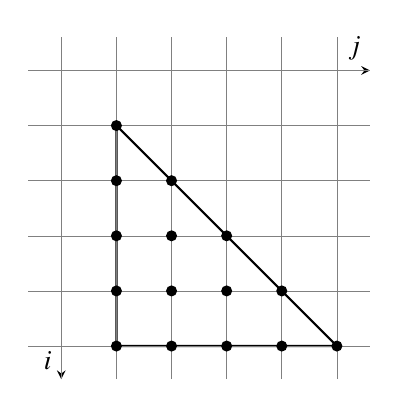
\begin{tikzpicture}[>=stealth,x=0.7cm,y=-0.7cm]
\draw[thick] (1,1)--(5,5)--(1,5)--(1,1);
\draw[->] (-0.6,0) to (5.6,0) node[anchor=south east] {$j$};
\draw[->] (0,-0.6) to (0,5.6) node[anchor=south east] {$i$};
\draw[help lines,step=0.7cm] (-0.6,5.6) grid (5.6,-0.6);
\foreach \i in {1,...,5}{
    \foreach \j in {1,...,\i}{
        \fill (\j,\i) circle (2pt);
    }
}
\end{tikzpicture}
\caption{The iteration domain of the loop nest in \autoref{f:loop nest}}
\label{f:iteration domain}
\end{figure}

Within the polyhedral model for analysis and transformation of
static affine programs, the most basic kind of set is the
\defindex{iteration domain}.
The iteration domain represents the iterations of a statement in a loop nest.
Take, for example, the loop nest in \autoref{f:loop nest}
and assume first that \lstinline{n} has a fixed value, say 5.
The pairs of values of \lstinline{i} and \lstinline{j} for
which statement \lstinline{S} is executed are shown graphically
in \autoref{f:iteration domain}.
Mathematically, this set of pairs can be represented as
$$
\{\,
(i,j) \in \ZZ^2 \mid 1 \le i \le 5 \wedge 1 \le j \le i
\,\}
$$
and the \isl/ notation is very similar:
\begin{lstlisting}[columns=flexible,escapechar=@,language=]{}
{ [i,j] : 1 <= i <= 5 and 1 <= j <= i }
\end{lstlisting}
In this notation,
the coordinates are separated by commas and enclosed in square
brackets.  This description of the space in which the set lives
is followed by a colon and the constraints on the coordinates.
Assuming the iterators are incremented by one in every iterations
of the loop, a lower and upper bound on each loop iterator
can be read off from the initialization and the test.
Note that in an \iscc/ set,
the coordinates are assumed to be integer by default.
For an iteration domain to be representable by such a set,
the iterators therefore need to be integers.

The constraints of a set need to be affine, i.e., linear plus constant term.
These affine constraint may be combined through conjunctions (\texttt{and}),
disjunctions (\texttt{or}), projections (\texttt{exists}) and
negations (\texttt{not}).
Note that the formula is immediately converted
into \indac{DNF}, so it may sometimes be more efficient
to construct a set from smaller sets by applying
basic operations such as intersection ({\tt *}),
union ({\tt +}) and difference ({\tt -}).
For example, the following square with its diagonal removed,
$$
\{\,
(i,j) \mid 0 \le i,j \le 10 \wedge \lnot (i = j)
\,\}
$$
can be constructed as
\begin{lstlisting}[columns=flexible,escapechar=@,language=]{}
{ [i,j] : 0 <= i,j <= 10 } - { [i,i] }
\end{lstlisting}
or as
\begin{lstlisting}[columns=flexible,escapechar=@,language=]{}
{ [i,j] : 0 <= i,j <= 10 and not (i = j) }
\end{lstlisting}
Note that an occurrence of a relational operator in a set description
may define several constraints, one for each pair of arguments.
The elements in a list of arguments are separated by a comma.
If there are no constraints on the coordinates, i.e., in case of
a universe set, the colon may be omitted as well.
For example
\begin{lstlisting}[columns=flexible,escapechar=@,language=]{}
{ [] }
\end{lstlisting}
represents the entire (unnamed) zero-dimensional space,
and should not be confused with
\begin{lstlisting}[columns=flexible,escapechar=@,language=]{}
{ }
\end{lstlisting}
which represents the empty set.

Returning to the iteration domain of the loop nest
in \autoref{f:loop nest}, we usually do not want to analyze
such a program for a specific value of \lstinline{n},
but instead for all possible values of \lstinline{n} at once.
A generic description of the iteration domain can be obtained
through the introduction of a (free) parameter, as in
\begin{lstlisting}[columns=flexible,escapechar=@,language=]{}
[n] -> { [i,j] : 1 <= i <= n and 1 <= j <= i }
\end{lstlisting}
The optional parameters should
be declared by placing them in a comma delimited list inside \lstinline![]!
(followed by an ``\lstinline!->!'') in front of the main set description.
The parameters are global and are identified by their names,
so the order inside the list is arbitrary.
This should be contrasted to the coordinates of a space, the names of
which are only relevant within the description of the set and which
are instead identified by their positions.
That is,
\begin{lstlisting}[columns=flexible,escapechar=@,language=]{}
[n] -> { [i,j] : 1 <= i <= n and 1 <= j <= i }
\end{lstlisting}
is equal to
\begin{lstlisting}[columns=flexible,escapechar=@,language=]{}
[n] -> { [a,b] : 1 <= a <= n and 1 <= b <= a }
\end{lstlisting}
but it is not equal to
\begin{lstlisting}[columns=flexible,escapechar=@,language=]{}
[n] -> { [j,i] : 1 <= i <= n and 1 <= j <= i }
\end{lstlisting}
(because the order of the coordinates has changed)
or
\begin{lstlisting}[columns=flexible,escapechar=@,language=]{}
[m] -> { [i,j] : 1 <= i <= m and 1 <= j <= i }
\end{lstlisting}
(because it involves a different parameter).

It is sometimes convenient to represent constraints that only
involve parameters and that are not tied to any particular space.
To construct such a parameter domain, the list of coordinates
should simply be omitted.  Note that the colon is required
in this case, even if there are no constraints.
In particular,
\begin{lstlisting}[columns=flexible,escapechar=@,language=]{}
{ : }
\end{lstlisting}
represents the universal parameter domain, which is very different
from the empty set.

To plug in a particular value for a parameter, the user should
take the \ai{intersection} (\ai[\tt]{*}) with a parameter domain
assigns a particular value to the parameter.
For example,
\begin{lstlisting}[columns=flexible,escapechar=@,language=]{}
S := [n] -> { [i,j] : 1 <= i <= n and 1 <= j <= i };
S * [n] -> { : n = 5 };
\end{lstlisting}
It should be noted, though, that the result is not the same
as simply replacing \lstinline{n} by 5 as the result of the above
sequence will still have the global parameter \lstinline{n} set to 5.
To avoid this assignment, the user should instead compute
the \ai{gist} (\ai[\tt]{\%}) of the original set in the context
of setting \lstinline{n} to 5.
That is, the result of the sequence below is \lstinline{True}.
\begin{lstlisting}[columns=flexible,escapechar=@,language=]{}
S1 := { [i,j] : 1 <= i <= 5 and 1 <= j <= i };
S2 := [n] -> { [i,j] : 1 <= i <= n and 1 <= j <= i };
(S2 % [n] -> { : n = 5}) = S1;
\end{lstlisting}

\begin{figure}
\begin{lstlisting}[escapechar=@]{}
for (i = 1; i <= n; i += 3)
    /* S */
\end{lstlisting}
\caption{A loop with non-unit stride}
\label{f:stride}
\end{figure}

If a loop has a non-unit stride as in \autoref{f:stride}
then affine constraints on the coordinates and the parameters
are not sufficient to represent the iteration domain.
What is needed is a way to express that the value of
\lstinline{i} is equal to 1 plus 3 times some integer and
this is where existentially quantified variables can be used.
Existentially quantified variables are introduced by the
\ai[\tt]{exists} keyword and followed by a colon.
They can only be used within a single disjunct.
As an example, the iteration domain of the loop in \autoref{f:stride}
can be represented as
\begin{lstlisting}[columns=flexible,escapechar=@,language=]{}
[n] -> { [i] : exists a : 1 <= i <= n and i = 1 + 3 a }
\end{lstlisting}

\begin{figure}
\begin{lstlisting}[escapechar=@]{}
for (i = 1; i <= n; ++i)
    if ((i + 1) % 5 <= 2)
	/* S */
\end{lstlisting}
\caption{A loop with a modulo condition}
\label{f:modulo}
\end{figure}

Existentially quantified variables are also useful to represent
modulo constraints.  Consider for example the loop in
\autoref{f:modulo}.  The iterator values \lstinline!i! for which
the statement \lstinline!S! is executed lie between
1 and \lstinline!n! and are such that the remainder of
\lstinline!i + 1! on division by 5 is less than or equal to 2.
The constraint $(i + 1) \bmod 5 \le 2$ can be written
as $(i + 1) - 5 \floor{\frac{i+1}5} \le 2$, where
$f = \floor{\frac{i+1}5}$ is the greatest integer part of $\frac{i+1}5$.
That is, $f$ is the unique integer value satisfying the constraints
$5 f \le i + 1$ and $5 f \ge (i+1) - 4$.
The iteration domain of the statement in \autoref{f:modulo}
can therefore be represented as
\begin{lstlisting}[columns=flexible,escapechar=@,language=]{}
[n] -> { [i] : exists f : 1 <= i <= n and (i + 1) - 5 f <= 2 and
	 (i + 1) - 4 <= 5 f <= i + 1 }
\end{lstlisting}
Since greatest integer parts occur relatively frequently, there is
a special notation for them in \isl/ using \lstinline![]!.
The above set can therefore also be represented as
\begin{lstlisting}[columns=flexible,escapechar=@,language=]{}
[n] -> { [i] : 1 <= i <= n and (i + 1) - 5 * [(i + 1)/5] <= 2 }
\end{lstlisting}
Actually, since modulos are pretty common too, \isl/ also has
a special notation for them and the set can therefore also be respresented as
\begin{lstlisting}[columns=flexible,escapechar=@,language=]{}
[n] -> { [i] : 1 <= i <= n and (i + 1) % 5 <= 2 }
\end{lstlisting}
It should be noted that \lstinline![]! always rounds down
(towards $-\infty$), while integer division in C truncates
(towards 0).  When translating conditions in C containing integer
divisions and/or modulos to \isl/ constraints, the user should therefore
make sure the sign of the dividend is positive.  If not, the integer
division needs to be translated differently for positive and negative
values.

\begin{figure}
\begin{lstlisting}[escapechar=@]{}
for (i = 0; i < n; ++i)
T:  t[i] = a[i];
for (i = 0; i < n; ++i)
    for (j = 0; j < n - i; ++j)
F:      t[j] = f(t[j], t[j+1]);
for (i = 0; i < n; ++i)
B:  b[i] = t[i];
\end{lstlisting}
\caption{A program with three loop nests}
\label{f:three loops}
\end{figure}

Most programs involve more than one statement.
Although it is possible to work with different sets, each
representing the iteration domain of a statement,
it is usually more convenient to collect all iteration domains
in a single set.  To be able to differentiate between iterations
of different statements with the same values for the iterators,
\isl/ allows spaces to be named.  The name is placed in front
of the \lstinline![]! enclosing the iterators.
Consider for example the program in \autoref{f:three loops}.
The program contains three statements which have been labeled
for convenience.
The iteration domain of the first statement (\lstinline!T!)
can be represented as
\begin{lstlisting}[columns=flexible,escapechar=@,language=]{}
[n] -> { T[i] : 0 <= i < n }
\end{lstlisting}
The union of all iteration domains can be represented as
\begin{lstlisting}[columns=flexible,escapechar=@,language=]{}
[n] -> {
    T[i] : 0 <= i < n;
    F[i,j] : 0 <= i < n and 0 <= j < n - i;
    B[i] : 0 <= i < n
}
\end{lstlisting}
The semicolon \lstinline{;} is used to express a disjunction
between spaces.  This should be contrasted with the \lstinline{or}
keyword which expresses a disjunction between conjunctions of constraints.
For example, the result of the following \iscc/ statement is
\lstinline{True}.
\begin{lstlisting}[columns=flexible,escapechar=@,language=]{}
{ [i] : i = 3 or i = 5 } = { [3]; [5] };
\end{lstlisting}

\subsubsection{Maps and Access Relations}

A second important concept in the polyhedral model is that
of an \defindex{access relation}.
An access relation connects iterations of a statement
to the array elements accessed by those iterations.
Such a binary relation can be represented by a map in \isl/.
Maps are defined in similar way to sets,
except that the single space is replaced by a pair of spaces separated
by \verb!->!.
As an example, consider once more the program in \autoref{f:three loops}.
In particular, consider the access \lstinline{t[j+1]} in
statement \lstinline{F}.
The index expression maps the pair of iterations \lstinline{i}
and \lstinline{j} to \lstinline{t[j+1]}, i.e., element \lstinline{j+1}
of a space with name \lstinline{t}.
Ignoring the loop bound constraints, this access relation can
be represented as
\begin{lstlisting}[columns=flexible,escapechar=@,language=]{}
{ F[i,j] -> t[j + 1] }
\end{lstlisting}
It is however customary to include the constraints on the iterators
in the access relation, resulting in
\begin{lstlisting}[columns=flexible,escapechar=@,language=]{}
[n] -> { F[i,j] -> t[j + 1] : 0 <= i < n and 0 <= j < n - i }
\end{lstlisting}
The constraints can be added by intersecting the domains
of the access relations with the iteration domains.
For example, the following sequence constructs the access
relation for all reads in the program.
\begin{lstlisting}[columns=flexible,escapechar=@,language=]{}
D := [n] -> {
    T[i] : 0 <= i < n;
    F[i,j] : 0 <= i < n and 0 <= j < n - i;
    B[i] : 0 <= i < n
};
Read := {
    T[i] -> a[i];
    F[i,j] -> t[j];
    F[i,j] -> t[j + 1];
    B[i] -> t[i]
};
Read := Read * D;
\end{lstlisting}
In this sequence, the \lstinline{*} operator, when applied
to a map and a set, intersects the domain of the map with the set.

The notation \lstinline{R(S)} can be used to compute the image
of the set \lstinline{S} under the map \lstinline{R}.
For example, given the sequence above, \lstinline!Read({F[0,1]})!
computes the array elements read in iteration $(0,1)$ of statement
\lstinline{F} and is equal to
\begin{lstlisting}[columns=flexible,escapechar=@,language=]{}
[n] -> { t[2] : n >= 2; t[1] : n >= 2 }
\end{lstlisting}
That is, elements 1 and 2 of the \lstinline{t} array are read,
provided \lstinline{n} is at least 2.

Maps need not be single-valued.
As an example, assume that \lstinline{A} is a two-dimensional
array of size \lstinline{n} in both dimensions.
Iterations \lstinline{i} of
a statement \lstinline{S} may pass a pointer to an entire row
of \lstinline{A} to a function as in \lstinline{f(A[i])}.
Without knowing anything about \lstinline{f}, we would have
to assume that this function may access any element of the row.
The access relation corresponding to \lstinline{A[i]} is therefore
\begin{lstlisting}[columns=flexible,escapechar=@,language=]{}
[n] -> { S[i] -> A[i,j] : 0 <= i,j < n }
\end{lstlisting}
This map associates \lstinline{n} elements of \lstinline{A}
to each iteration of \lstinline{S}.

\subsubsection{Nested Spaces}

Each space may contain a nested pair of spaces.  Such nested spaces
are extremely useful in more advanced applications.
As an example, suppose that during equivalence checking
\shortcite{Verdoolaege2009equivalence}
of two programs the iterations of \verb!S1! in one program are supposed to
produce the same results as the same iterations of \verb!SA! in the other program,
which may be described using the following map
\begin{verbatim}
[n] -> { S1[i] -> SA[i] : 0 <= i <= n }
\end{verbatim}
If the iterations of \verb!S1! depend on the same iterations
of \verb!S2!, i.e., \verb!{S1[i]->S2[i]}!, while those of \verb!SA!
depend on the next iteration of \verb!B!, i.e., \verb!{SA[i]->SB[i+1]}!,
then we can apply the cross product of these two dependence maps, i.e.,
\begin{verbatim}
{ [S1[i] -> SA[i']] -> [S2[i] -> SB[1+i']] }
\end{verbatim}
to the original map to find
out which iterations of \verb!S2! should correspond to which
iterations of \verb!SB!.

\subsubsection{Basic Operations}

Basic operations on sets and maps include intersection (\ai[\tt]{*}),
union (\ai[\tt]{+}), difference (\ai[\tt]{-}), cross product (\ai[\tt]{cross}),
sampling (\ai[\tt]{sample}), affine hull (\ai[\tt]{aff}),
lexicographic optimization (\ai[\tt]{lexmin} or \ai[\tt]{lexmax}),
subset (\ai[\tt]{<=}) and equality (\ai[\tt]{=}) tests,
code generation (\ai[\tt]{codegen})
and the cardinality (\ai[\tt]{card}).
Additional operations on maps include computing domain (\ai[\tt]{dom})
and range (\ai[\tt]{ran}), differences between image and domain (\ai[\tt]{deltas}),
join (\ai[\tt]{.}), inverse (\ai[\tt]{\^{}-1}) and transitive closure (\ai[\tt]{\^{}+}).
The latter may result in an overapproximation.

The \ai[\tt]{card} operation computes the number of elements in a set
or the number of elements in the image of a domain element of a map.
The operation is performed exactly and completely symbolically and
the result is a piecewise quasipolynomial, i.e., a subdivision of one
or more spaces, with a quasipolynomial associated to each cell in the subdivision.
As a trivial example, the result of
\begin{verbatim}
card { A[i] -> B[j] : 0 <= j <= i }
\end{verbatim}
is \verb!{ A[i] -> (1+i) : i >= 0 }!.
Operations on piecewise quasipolynomials include sum (\ai[\tt]{+})
and difference (\ai[\tt]{-}) and the computation of an upper bound over the domain.
If the domain contains a pair of nested spaces, then the upper bound is computed over
the nested range.  As another trivial example, the result of
\begin{verbatim}
ub{ [[i] -> [j]] -> j^2 : -i <= j <= i }
\end{verbatim}
is
\verb!({ [i] -> max(i^2) : i >= 0 }, True)!.
The first element in this list is the actual bound in the form
of a piecewise quasipolynomial fold,
i.e., a maximum of quasipolynomials defined over cells.
The second indicates whether the bound is tight, i.e., whether
a maximum has been computed.

\subsubsection{Advanced Operations}

While the basic {\tt card} operation simply counts the number of elements
in an affine set, it is also possible to assign a weight to each element
of the set and to compute the sum of those weights over all the points in the set.
The syntax for this weighted counting is to compute the {\tt sum} of
a piecewise quasipolynomial over its domain.  As in the case of the {\tt ub}
operator, if the domain contains a pair of nested space, the sum is computed
over the range.  As an example, the result
of
\begin{verbatim}
sum{ [[i] -> [j]] -> i*j : 0 <= j <= i }
\end{verbatim}
is
\verb|{ [i] -> (1/2*i^2+1/2*i^3) : i >= 0 }|.

After the computation of some sum or bound, the result may have to
be reformulated in terms of other variables.  For example, during
inter procedural analysis, a result computed in terms of the formal
parameters may have to be reformulated in terms of the actual parameters.
{\tt iscc} therefore allows maps and
piecewise quasipolynomials or folds to be composed.
If the map is multi-valued, then the composition maps each domain element
to the sum or upper bound of the values at its image elements.

Finally, because of its high-level representation, {\tt iscc} can
provide a dependence analysis operation taking only three maps as input,
the sink accesses, the potential source accesses and a schedule.
The result is a single dependence map.


\subsubsection{More Examples}
\begin{verbatim}
P := [n, m] -> { [i,j] : 0 <= i <= n and i <= j <= m };
card P;

f := [n,m] -> { [i,j] -> i*j + n*i*i*j : i,j >= 0 and 5i + 27j <= n+m };
sum f;
s := sum f;
s @ [n,m] -> { : 0 <= n,m <= 20 };

f := [n] -> { [i] -> 2*n*i - n*n + 3*n - 1/2*i*i - 3/2*i-1 :
                (exists j : 0 <= i < 4*n-1 and 0 <= j < n and
                            2*n-1 <= i+j <= 4*n-2 and i <= 2*n-1 ) };
ub f;
u := (ub f)[0];
u @ [n] -> { : 0 <= n <= 10 };

m := [n] -> { [i,j] -> [i+1,j+1] : 1 <= i,j < n;
              [i,j] -> [i+1,j-1] : 1 <= i < n and 2 <= j <= n };
m^+;
(m^+)[0];

codegen [N] -> { A[i] -> [i,0] : 0 <= i <= N; B[i] -> [i,1] : 1 <= i <= N };

{ [k] -> [i] : 1 <= i <= k } . { [n] -> 2 * n : n >= 1 };

{ [m] -> [c] : 1 <= c <= m } . { [k] -> max((3 * k + k^2)) : k >= 1 };
\end{verbatim}

\subsubsection{Comparison to other Interactive Polyhedral Tools}

Two related interactive polyhedral tools are
the Omega calculator \shortcite{Omega_calc}
and {\tt SPPoC} \shortcite{Boulet2001SPPoC}.
The syntax of {\tt iscc} was very much inspired
by that of the Omega calculator.  However, the Omega
calculator only knows sets and maps.  In particular,
it does not perform any form of counting.  An earlier version
of \barvinok/ came with a modified version of
the Omega calculator that introduced an operation
for counting the number of elements in a set, but it
would simply print the result and not allow any further
manipulations.
{\tt SPPoC} does support counting, but only the basic
operation of counting the elements in a set.
In particular, it does not support weighted counting,
nor the computation of upper bounds.
It also only supports (single-valued) functions
and not generic relations like the Omega calculator and {\tt iscc}.
Internally, {\tt SPPoC} uses {\tt PolyLib}, {\tt PipLib} and {\tt omega}
to perform
its operations.  Although the first two of these libraries may have been
state-of-the-art at the time {\tt SPPoC} was created, they are
no longer actively maintained and have been largely
superseded by more recent libraries.
In particular, {\tt PipLib} effectively only supports a single
operation, which is now also available in both {\tt isl} and {\tt PPL}.
The operations on rational polyhedra in {\tt PolyLib} are also
available in {\tt PPL}, usually through a cleaner interface and
with a more efficient implementation.  As to counting the elements
in a parametric polytope, Barvinok's algorithm,
implemented in the {\tt barvinok} library, is usually much faster
than the algorithm implemented in {\tt PolyLib}
\shortcite{Verdoolaege2007parametric}.
Furthermore,
the ability to work with named and nested spaces and the ability
of sets and maps to contain (pairs of) elements from different spaces
are not available in the Omega calculator and {\tt SPPoC}.

\newpage
\tablecaption{{\tt iscc} operations.  The variables
have the following types,
$s$: set,
$m$: map,
$q$: piecewise quasipolynomial,
$f$: piecewise quasipolynomial fold,
$t$: schedule (tree),
$l$: list,
$i$: integer,
$b$: boolean,
$S$: string,
$o$: object of any type
}
\label{t:iscc}
\tablehead{
\hline
Syntax & Meaning
\\
\hline
}
\tabletail{
\multicolumn{2}{r}{\small\sl continued on next page}
\\
}
\tablelasttail{}
\begin{supertabular}{p{0.35\textwidth}p{0.6\textwidth}}
$s_2$ := \ai[\tt]{aff} $s_1$ & affine hull of $s_1$
\\
$m_2$ := \ai[\tt]{aff} $m_1$ & affine hull of $m_1$
\\
$q$ := \ai[\tt]{card} $s$ &
number of elements in the set $s$
\\
$q$ := \ai[\tt]{card} $m$ &
number of elements in the image of a domain element
\\
$s_2$ := \ai[\tt]{coalesce} $s_1$ &
simplify the representation of set $s_1$ by trying
to combine pairs of basic sets into a single
basic set
\\
$m_2$ := \ai[\tt]{coalesce} $m_1$ &
simplify the representation of map $m_1$ by trying
to combine pairs of basic maps into a single
basic map
\\
$q_2$ := \ai[\tt]{coalesce} $q_1$ &
simplify the representation of $q_1$ by trying
to combine pairs of basic sets in the domain
of $q_1$ into a single basic set
\\
$f_2$ := \ai[\tt]{coalesce} $f_1$ &
simplify the representation of $f_1$ by trying
to combine pairs of basic sets in the domain
of $f_1$ into a single basic set
\\
\ai[\tt]{codegen} $t$ &
generate code for the given schedule.
\\
\ai[\tt]{codegen} $m$ &
generate code for the given schedule.
\\
\ai[\tt]{codegen} $m_1$ \ai[\tt]{using} $m_2$ &
generate code for the schedule $m_1$ using the options $m_2$.
\\
$s_2$ := \ai[\tt]{coefficients} $s_1$ &
The set of coefficients of valid constraints for $s_1$
\\
$s_2$ := \ai[\tt]{solutions} $s_1$ &
The set of elements satisfying the constraints with coefficients in $s_1$
\\
$s_3$ := $s_1$ \ai[\tt]{cross} $s_2$ &
Cartesian product of $s_1$ and $s_2$
\\
$m_3$ := $m_1$ \ai[\tt]{cross} $m_2$ &
Cartesian product of $m_1$ and $m_2$
\\
$m_3$ := $m_1$ \ai[\tt]{cross\_range} $m_2$ &
Cartesian product of the ranges of $m_1$ and $m_2$ for their shared domain
\\
$s$ := \ai[\tt]{deltas} $m$ &
the set $\{\, y - x \mid x \to y \in m \,\}$
\\
$m_2$ := \ai[\tt]{deltas\_map} $m_1$ &
the map $\{\, (x \to y) \to y - x \mid x \to y \in m_1 \,\}$
\\
$s$ := \ai[\tt]{dom} $m$ &
domain of map $m$
\\
$s$ := \ai[\tt]{dom} $q$ &
domain of piecewise quasipolynomial $q$
\\
$s$ := \ai[\tt]{dom} $f$ &
domain of piecewise quasipolynomial fold $f$
\\
$s$ := \ai[\tt]{dom} $t$ &
domain of schedule $t$
\\
$s$ := \ai[\tt]{domain} $m$ &
domain of map $m$
\\
$s$ := \ai[\tt]{domain} $q$ &
domain of piecewise quasipolynomial $q$
\\
$s$ := \ai[\tt]{domain} $f$ &
domain of piecewise quasipolynomial fold $f$
\\
$s$ := \ai[\tt]{domain} $t$ &
domain of schedule $t$
\\
$m_2$ := \ai[\tt]{domain\_map} $m_1$ &
a map from a wrapped copy of $m_1$ to the domain of $m_1$
\\
$s$ := \ai[\tt]{ran} $m$ &
range of map $m$
\\
$s$ := \ai[\tt]{range} $m$ &
range of map $m$
\\
$m_2$ := \ai[\tt]{range\_map} $m_1$ &
a map from a wrapped copy of $m_1$ to the range of $m_1$
\\
$m$ := \ai[\tt]{identity} $s$ &
identity relation on $s$
\\
$q$ := \ai[\tt]{lattice\_width} $s$ &
lattice width of the set $s$
\\
$l$ := \ai[\tt]{lb} $q$ &
compute a
lower bound on the piecewise quasipolynomial $q$ over
all integer points in the domain of $q$
and return a list containing the lower bound
and a boolean that is true if the lower bound
is known to be tight.
If the domain of $q$ wraps a map, then the lower
bound is computed over all integer points in
the range of the wrapped map instead.
\\
$s_2$ := \ai[\tt]{lexmin} $s_1$ &
lexicographically minimal element of $s_1$
\\
$m_2$ := \ai[\tt]{lexmin} $m_1$ &
lexicographically minimal image element
\\
$s_2$ := \ai[\tt]{lexmax} $s_1$ &
lexicographically maximal element of $s_1$
\\
$m_2$ := \ai[\tt]{lexmax} $m_1$ &
lexicographically maximal image element
\\
$s_2$ := \ai[\tt]{lift} $s_1$ &
lift $s_1$ to a space with extra dimensions corresponding
to the existentially quantified variables in $s_1$ such
that \lstinline!domain(unwrap(lift S))! is equal to \lstinline!S!
\\
$m$ := \ai[\tt]{map} $t$ &
convert schedule $t$ to a map representation
\\
$s_2$ := \ai[\tt]{params} $s_1$ &
parameter domain of set $s_1$
\\
$s$ := \ai[\tt]{params} $m$ &
parameter domain of map $m$
\\
$l$ := \ai[\tt]{parse\_file} $S$ &
parse the file names $S$ and return a list consisting of
the iteration domain, the must write access relation,
the may write access relation, the read access relation and
the original schedule.
This operation is only available if \ai[\tt]{pet}
support was compiled in.
\\
$s_2$ := \ai[\tt]{poly} $s_1$ & polyhedral hull of $s_1$
\\
$m_2$ := \ai[\tt]{poly} $m_1$ & polyhedral hull of $m_1$
\\
$q_2$ := \ai[\tt]{poly} $q_1$ & polynomial approximation of $q_1$
\\
$q_2$ := \ai[\tt]{lpoly} $q_1$ & polynomial underapproximation of $q_1$
\\
$q_2$ := \ai[\tt]{upoly} $q_1$ & polynomial overapproximation of $q_1$
\\
$l$ := \ai[\tt]{pow} $m$\ &
compute an overapproximation of the power
of $m$ and return a list containing the overapproximation
and a boolean that is true if the overapproximation
is known to be exact
\\
\ai[\tt]{print} $o$ &
print object
\\
$o$ := \ai[\tt]{read} {\tt "}{\it filename}{\tt"} &
read object from file
\\
$s_2$ := \ai[\tt]{sample} $s_1$ &
a sample element of the set $s_1$
\\
$m_2$ := \ai[\tt]{sample} $m_1$ &
a sample element of the map $m_1$
\\
$s_2$ := \ai[\tt]{scan} $s_1$ &
the set $s_1$ split into individual elements,
provided $s_1$ contains a finite number of elements
\\
$m_2$ := \ai[\tt]{scan} $m_1$ &
the map $m_1$ split into individual elements,
provided $m_1$ contains a finite number of elements
\\
\ai[\tt]{source} {\tt "}{\it filename}{\tt"} &
read commands from file
\\
$q_2$ := \ai[\tt]{sum} $q_1$ &
sum $q_1$ over all integer points in the domain of $q_1$,
or, if the domain of $q_1$ wraps a map, over all integer
points in the range of the wrapped map.
\\
$S$ := \ai[\tt]{typeof} $o$ &
a string representation of the type of $o$
\\
$l$ := \ai[\tt]{ub} $q$ &
compute an
upper bound on the piecewise quasipolynomial $q$ over
all integer points in the domain of $q$
and return a list containing the upper bound
and a boolean that is true if the upper bound
is known to be tight.
If the domain of $q$ wraps a map, then the upper
bound is computed over all integer points in
the range of the wrapped map instead.
\\
$l$ := \ai[\tt]{vertices} $s$ &
a list of vertices of the rational polytope defined by the same constraints
as $s$
\\
$s$ := \ai[\tt]{wrap} $m$ &
wrap the map in a set
\\
$m$ := \ai[\tt]{unwrap} $s$ &
unwrap the map from the set
\\
\ai[\tt]{write} {\tt "}{\it filename}{\tt"} $o$ &
write object to file
\\
$m_2$ := \ai[\tt]{zip} $m_1$ &
the cross product of domain and range of $m_1$, i.e.,
$\{\, (\vec w \to \vec y) \to (\vec x \to \vec z)
\mid (\vec w \to \vec x) \to (\vec y \to \vec z) \in m_1 \,\}$
\\
$m_3$ := \ai[\tt]{any} $m_1$ \ai[\tt]{before} $m_2$ \ai[\tt]{under} $t$ &
compute a map from any element $x$ in the domain of $m_1$
to any element $y$ in the domain of $m_2$
such that their images $m_1(x)$ and $m_2(y)$ overlap
and such that $x$ is scheduled before $y$ by $t$.
\\
$m_4$ := \ai[\tt]{any} $m_1$ \ai[\tt]{before} $m_2$ \ai[\tt]{under} $m_3$ &
same as the previous operation, with the schedule represented by a map.
\\
$l$ := \ai[\tt]{last} $m_1$ \ai[\tt]{before} $m_2$ \ai[\tt]{under} $t$ &
compute a map that contains for any element $y$ in the domain of $m_2$
a mapping from the last element $x$ in the domain of $m_1$
(according to the schedule $t$) to $y$
such that $m_1(x)$ and $m_2(y)$ overlap
and such that $x$ is scheduled before $y$ by $t$.
Return a list containing this map and the subset of
$m_2$ for which there is no corresponding element in the domain of $m_1$.
\\
$l$ := \ai[\tt]{last} $m_1$ \ai[\tt]{before} $m_2$ \ai[\tt]{under} $m_3$ &
same as the previous operation, with the schedule represented by a map.
\\
$m_4$ := \ai[\tt]{any} $m_1$ \ai[\tt]{last} $m_2$ \ai[\tt]{before} $m_3$
\ai[\tt]{under} $t$ &
compute a map that contains for any element $y$ in the domain of $m_3$
a mapping from the last element $x$ in the domain of $m_2$
(according to the schedule $t$) to $y$
such that $m_2(x)$ and $m_3(y)$ overlap
and such that $x$ is scheduled before $y$ by $t$
as well as from any element $z$ in the domain of $m_1$ such that
$m_1(z)$ and $m_3(y)$ overlap,
$z$ is scheduled before $y$ by $t$
and such that there is no $x$ in the domain of $m_2$ with
$m_2(x) \cap m_3(y) \ne \emptyset$ and
$x$ scheduled between $z$ and $y$ by $t$.
\\
$m_5$ := \ai[\tt]{any} $m_1$ \ai[\tt]{last} $m_2$ \ai[\tt]{before} $m_3$
\ai[\tt]{under} $m_4$ &
same as the previous operation, with the schedule represented by a map.
\\
$t$ := \ai[\tt]{schedule} $s$ \ai[\tt]{respecting} $m_1$ \ai[\tt]{minimizing} $m_2$ &
compute a schedule for the domains in $s$ that respects all dependences
in $m_1$ and tries to minimize the dependences in $m_2$.
\\
$b_3$ := $b_1$ \ai{$+$} $b_2$ & or
\\
$i_3$ := $i_1$ \ai{$+$} $i_2$ & sum
\\
$s_3$ := $s_1$ \ai{$+$} $s_2$ & union
\\
$m_3$ := $m_1$ \ai{$+$} $m_2$ & union
\\
$q_3$ := $q_1$ \ai{$+$} $q_2$ & sum
\\
$f_2$ := $f_1$ \ai{$+$} $q$ & sum
\\
$f_2$ := $q$ \ai{$+$} $f_1$ & sum
\\
$S_3$ := $S_1$ \ai{$+$} $S_2$ & concatenation
\\
$S_2$ := $o$ \ai{$+$} $S_1$ &
concatenation of stringification of $o$ and $S_1$
\\
$S_2$ := $S_1$ \ai{$+$} $o$ &
concatenation of $S_1$ and stringification of $o$
\\
$i_3$ := $i_1$ \ai{$-$} $i_2$ & difference
\\
$s_3$ := $s_1$ \ai{$-$} $s_2$ & set difference
\\
$m_3$ := $m_1$ \ai{$-$} $m_2$ & set difference
\\
$m_2$ := $m_1$ \ai{$-$} $s$ & subtract $s$ from the domain of $m_1$
\\
$m_2$ := $m_1$ \ai[\tt]{->-} $s$ & subtract $s$ from the range of $m_1$
\\
$q_3$ := $q_1$ \ai{$-$} $q_2$ & difference
\\
$b_3$ := $b_1$ \ai{$*$} $b_2$ & and
\\
$i_3$ := $i_1$ \ai{$*$} $i_2$ & product
\\
$s_3$ := $s_1$ \ai{$*$} $s_2$ & intersection
\\
$m_3$ := $m_1$ \ai{$*$} $m_2$ & intersection
\\
$q_2$ := $i$ \ai{$*$} $q_1$ & product
\\
$q_2$ := $q_1$ \ai{$*$} $i$ & product
\\
$q_3$ := $q_1$ \ai{$*$} $q_2$ & product
\\
$f_2$ := $i$ \ai{$*$} $f_1$ & product
\\
$f_2$ := $f_1$ \ai{$*$} $i$ & product
\\
$m_2$ := $m_1$ \ai{$*$} $s$ & intersect domain of $m_1$ with $s$
\\
$q_2$ := $q_1$ \ai{$*$} $s$ & intersect domain of $q_1$ with $s$
\\
$f_2$ := $f_1$ \ai{$*$} $s$ & intersect domain of $f_1$ with $s$
\\
$m_2$ := $m_1$ \ai[\tt]{->$*$} $s$ & intersect range of $m_1$ with $s$
\\
$s_2$ := $m$($s_1$) & apply map $m$ to set $s_1$
\\
$q_2$ := $q_1$($s$) & apply $q_1$ to each element in $s$ and compute
the sum of the results
\\
$l$ := $f$($s$) & apply $f$ to each element in $s$, compute
a bound of the results
and return a list containing the bound
and a boolean that is true if the bound
is known to be tight.
\\
$m_3$ := $m_1$ \ai[\tt]{.} $m_2$ & join of $m_1$ and $m_2$
\\
$m_3$ := $m_1$ \ai[\tt]{before} $m_2$ & join of $m_1$ and $m_2$
\\
$m_3$ := $m_2$($m_1)$ & join of $m_1$ and $m_2$
\\
$m_3$ := $m_2$ \ai[\tt]{after} $m_1$ & join of $m_1$ and $m_2$
\\
$f_3$ := $f_1$ \ai[\tt]{.} $f_2$ & join of $f_1$ and $f_2$, combining
the lists of quasipolynomials over shared domains
\\
$q_2$ := $m$ \ai[\tt]{.} $q_1$ & join of $m$ and $q_1$, taking the sum
over all elements in the intersection of the range of $m$ and the domain
of $q_1$
\\
$q_2$ := $m$ \ai[\tt]{before} $q_1$ & $q_2$ := $m$ \ai[\tt]{.} $q_1$
\\
$q_2$ := $q_1(m)$ & $q_2$ := $m$ \ai[\tt]{.} $q_1$
\\
$q_2$ := $q_1$ \ai[\tt]{after} $m$ & $q_2$ := $m$ \ai[\tt]{.} $q_1$
\\
$l$ := $m$ \ai[\tt]{.} $f$ & join of $m$ and $f$, computing a bound
over all elements in the intersection of the range of $m$ and the domain
of $f$ and returning a list containing the bound
and a boolean that is true if the bound is known to be tight.
\\
$l$ := $m$ \ai[\tt]{before} $f$ & $l$ := $m$ \ai[\tt]{.} $f$
\\
$l$ := $f(m)$ & $l$ := $m$ \ai[\tt]{.} $f$
\\
$l$ := $f$ \ai[\tt]{after} $m$ & $l$ := $m$ \ai[\tt]{.} $f$
\\
$m$ := $s_1$ \ai[\tt]{->} $s_2$ & universal map with domain $s_1$
and range $s_2$
\\
$q_2$ := $q_1$ \ai{@} $s$ &
evaluate the piecewise quasipolynomial $q_1$ in each element
of the set $s$ and return a piecewise quasipolynomial
mapping each of the individual elements to the resulting
constant
\\
$q$ := $f$ \ai{@} $s$ &
evaluate the piecewise quasipolynomial fold $f$ in each element
of the set $s$ and return a piecewise quasipolynomial
mapping each of the individual elements to the resulting
constant
\\
$s_3$ := $s_1$ \ai[\tt]{\%} $s_2$ &
simplify $s_1$ in the context of $s_2$, i.e., compute
the gist of $s_1$ given $s_2$
\\
$m_3$ := $m_1$ \ai[\tt]{\%} $m_2$ &
simplify $m_1$ in the context of $m_2$, i.e., compute
the gist of $m_1$ given $m_2$
\\
$m_2$ := $m_1$ \ai[\tt]{\%} $s$ &
simplify $m_1$ in the context of the domain $s$, i.e., compute
the gist of $m_1$ given domain $s$
\\
$q_2$ := $q_1$ \ai[\tt]{\%} $s$ &
simplify $q_1$ in the context of the domain $s$, i.e., compute
the gist of $q_1$ given $s$
\\
$f_2$ := $f_1$ \ai[\tt]{\%} $s$ &
simplify $f_1$ in the context of the domain $s$, i.e., compute
the gist of $f_1$ given $s$
\\
$m_2$ := $m_1$\ai[\tt]{\^{}}i & the $i$th power of $m_1$;
if $i$ is negative then the result is the ($-i$)th power of the inverse
of $m_1$
\\
$l$ := $m$\ai[\tt]{\^{}+} &
compute an overapproximation of the transitive closure
of $m$ and return a list containing the overapproximation
and a boolean that is true if the overapproximation
is known to be exact
\\
$o$ := $l$[$i$] &
the element at position $i$ in the list $l$
\\
$b$ := $q_1$ \ai[\tt]{==} $q_2$ & is $q_1$ obviously equal to $q_2$?
\\
$b$ := $f_1$ \ai[\tt]{==} $f_2$ & is $f_1$ obviously equal to $f_2$?
\\
$b$ := $s_1$ \ai[\tt]{=} $s_2$ & is $s_1$ equal to $s_2$?
\\
$b$ := $m_1$ \ai[\tt]{=} $m_2$ & is $m_1$ equal to $m_2$?
\\
$b$ := $S_1$ \ai[\tt]{=} $S_2$ & is $S_1$ equal to $S_2$?
\\
$b$ := $s_1$ \ai[\tt]{<=} $s_2$ & is $s_1$ a subset of $s_2$?
\\
$b$ := $m_1$ \ai[\tt]{<=} $m_2$ & is $m_1$ a subset of $m_2$?
\\
$b$ := $s_1$ \ai[\tt]{<} $s_2$ & is $s_1$ a proper subset of $s_2$?
\\
$b$ := $m_1$ \ai[\tt]{<} $m_2$ & is $m_1$ a proper subset of $m_2$?
\\
$b$ := $s_1$ \ai[\tt]{>=} $s_2$ & is $s_1$ a superset of $s_2$?
\\
$b$ := $m_1$ \ai[\tt]{>=} $m_2$ & is $m_1$ a superset of $m_2$?
\\
$b$ := $s_1$ \ai[\tt]{>} $s_2$ & is $s_1$ a proper superset of $s_2$?
\\
$b$ := $m_1$ \ai[\tt]{>} $m_2$ & is $m_1$ a proper superset of $m_2$?
\\
$m$ := $s_1$ \ai[\tt]{<<} $s_2$ & a map from
$s_1$ to $s_2$ of those elements that live in the same space and
such that the elements of $s_1$ are lexicographically strictly smaller
than those of $s_2$.
\\
$m_3$ := $m_1$ \ai[\tt]{<<} $m_2$ & a map from the domain of
$m_1$ to the domain of $m_2$ of those elements such that their images
live in the same space and such that the images of the elements of
$m_1$ are lexicographically strictly smaller than those of $m_2$.
\\
$m$ := $s_1$ \ai[\tt]{<<=} $s_2$ & a map from
$s_1$ to $s_2$ of those elements that live in the same space and
such that the elements of $s_1$ are lexicographically smaller
than those of $s_2$.
\\
$m_3$ := $m_1$ \ai[\tt]{<<=} $m_2$ & a map from the domain of
$m_1$ to the domain of $m_2$ of those elements such that their images
live in the same space and such that the images of the elements of
$m_1$ are lexicographically smaller than those of $m_2$.
\\
$m$ := $s_1$ \ai[\tt]{>>} $s_2$ & a map from
$s_1$ to $s_2$ of those elements that live in the same space and
such that the elements of $s_1$ are lexicographically strictly greater
than those of $s_2$.
\\
$m_3$ := $m_1$ \ai[\tt]{>>} $m_2$ & a map from the domain of
$m_1$ to the domain of $m_2$ of those elements such that their images
live in the same space and such that the images of the elements of
$m_1$ are lexicographically strictly greater than those of $m_2$.
\\
$m$ := $s_1$ \ai[\tt]{>>=} $s_2$ & a map from
$s_1$ to $s_2$ of those elements that live in the same space and
such that the elements of $s_1$ are lexicographically greater
than those of $s_2$.
\\
$m_3$ := $m_1$ \ai[\tt]{>>=} $m_2$ & a map from the domain of
$m_1$ to the domain of $m_2$ of those elements such that their images
live in the same space and such that the images of the elements of
$m_1$ are lexicographically greater than those of $m_2$.
\\
\end{supertabular}


\section{\protect\PolyLib/ interface of the \protect\ai[\tt]{barvinok} library
(obsolescent)}

Although \barvinok/ currently still uses \PolyLib/ internally,
this is likely to change in the not too distant future.
Consider using \isl/ based alternatives for the functions in this section
as the latter are likely to be removed in future releases.

Our \barvinok/ library is built on top of \PolyLib/ 
\shortcite{Wilde1993,Loechner1999}.
In particular, it reuses the implementations
of the algorithm of 
\shortciteN{Loechner97parameterized}
for computing parametric vertices
and the algorithm of
\shortciteN{Clauss1998parametric}
for computing chamber decompositions.
Initially, our library was meant to be a replacement
for the algorithm of \shortciteN{Clauss1998parametric},
also implemented in \PolyLib/, for computing quasi-polynomials.
To ease the transition of application programs we
tried to reuse the existing data structures as much as possible.

\subsection{Existing Data Structures}
\label{a:existing}

Inside \PolyLib/ integer values are represented by the 
\ai[\tt]{Value} data type.
Depending on a configure option, the data type may
either by a 32-bit integer, a 64-bit integer
or an arbitrary precision integer using \ai[\tt]{GMP}.
The \barvinok/ library requires that \PolyLib/ is compiled
with support for arbitrary precision integers.

The basic structure for representing (unions of) polyhedra is a
\ai[\tt]{Polyhedron}.
\begin{verbatim}
typedef struct polyhedron {
  unsigned Dimension, NbConstraints, NbRays, NbEq, NbBid;
  Value **Constraint;
  Value **Ray;
  Value *p_Init;
  int p_Init_size;
  struct polyhedron *next;
} Polyhedron;
\end{verbatim}
The attribute \ai[\tt]{Dimension} is the dimension
of the ambient space, i.e., the number of variables.
The attributes \ai[\tt]{Constraint}
and \ai[\tt]{Ray} point to two-dimensional arrays
of constraints and generators, respectively.
The number of rows is stored in
\ai[\tt]{NbConstraints} and
\ai[\tt]{NbRays}, respectively.
The number of columns in both arrays is equal
to \verb!1+Dimension+1!.
The first column of \ai[\tt]{Constraint} is either
$0$ or $1$ depending on whether the constraint 
is an equality ($0$) or an inequality ($1$).
The number of equalities is stored in \ai[\tt]{NbEq}.
If the constraint is $\sp a x + c \ge 0$, then
the next columns contain the coefficients $a_i$
and the final column contains the constant $c$.
The first column of \ai[\tt]{Ray} is either
$0$ or $1$ depending on whether the generator 
is a line ($0$) or a vertex or ray ($1$).
The number of lines is stored in \ai[\tt]{NbBid}.
Let $d$ be the \ac{lcm} of the denominators of the coordinates
of a vertex $\vec v$, then the next columns contain
$d v_i$ and the final column contains $d$.
For a ray, the final column contains $0$.
The field \ai[\tt]{next} points to the next polyhedron in
the union of polyhedra.
It is \verb+0+ if this is the last (or only) polyhedron in the union.
For more information on this structure, we refer to \shortciteN{Wilde1993}.

Quasi-polynomials are represented using the 
\ai[\tt]{evalue} and \ai[\tt]{enode} structures.
\begin{verbatim}
typedef enum { polynomial, periodic, evector } enode_type;

typedef struct _evalue {
  Value d;              /* denominator */
  union {
    Value n;            /* numerator (if denominator != 0) */
    struct _enode *p;   /* pointer   (if denominator == 0) */
  } x;
} evalue;

typedef struct _enode {
  enode_type type;      /* polynomial or periodic or evector */
  int size;             /* number of attached pointers */
  int pos;              /* parameter position */
  evalue arr[1];        /* array of rational/pointer */
} enode;
\end{verbatim}
If the field \ai[\tt]{d} of an \ai[\tt]{evalue} is zero, then
the \ai[\tt]{evalue} is a placeholder for a pointer to
an \ai[\tt]{enode}, stored in \ai[\tt]{x.p}.
Otherwise, the \ai[\tt]{evalue} is a rational number with
numerator \ai[\tt]{x.n} and denominator \ai[\tt]{d}.
An \ai[\tt]{enode} is either a \ai[\tt]{polynomial}
or a \ai[\tt]{periodic}, depending on the value
of \ai[\tt]{type}.
The length of the array \ai[\tt]{arr} is stored in \ai[\tt]{size}.
For a \ai[\tt]{polynomial}, \ai[\tt]{arr} contains the coefficients.
For a \ai[\tt]{periodic}, it contains the values for the different
residue classes modulo the parameter indicated by \ai[\tt]{pos}.
For a polynomial, \ai[\tt]{pos} refers to the variable
of the polynomial.
The value of \ai[\tt]{pos} is \verb+1+ for the first parameter.
That is, if the value of \ai[\tt]{pos} is \verb+1+ and the first
parameter is $p$, and if the length of the array is $l$,
then in case it is a polynomial, the
 \ai[\tt]{enode} represents
$$
\verb+arr[0]+ + \verb+arr[1]+ p + \verb+arr[2]+ p^2 + \cdots +
\verb+arr[l-1]+ p^{l-1}
.
$$
If it is a periodic, then it represents
$$
\left[
\verb+arr[0]+, \verb+arr[1]+,  \verb+arr[2]+, \ldots,
\verb+arr[l-1]+
\right]_p
.
$$
Note that the elements of a \ai[\tt]{periodic} may themselves
be other \ai[\tt]{periodic}s or even \ai[\tt]{polynomial}s.
In our library, we only allow the elements of a  \ai[\tt]{periodic}
to be other \ai[\tt]{periodic}s or rational numbers.
The chambers and their corresponding quasi-polynomial are
stored in \ai[\tt]{Enumeration} structures.
\begin{verbatim}
typedef struct _enumeration {
  Polyhedron *ValidityDomain; /* constraints on the parameters */
  evalue EP;                  /* dimension = combined space    */
  struct _enumeration *next;  /* Ehrhart Polynomial,
                                 corresponding to parameter
                                 values inside the domain
                                 ValidityDomain above          */
} Enumeration;
\end{verbatim}
For more information on these structures, we refer to \shortciteN{Loechner1999}.

\begin{example}
Figure~\ref{f:Loechner} is a skillful reconstruction
of Figure~2 from \shortciteN{Loechner1999}.
It shows the contents of the \ai[\tt]{enode} structures
representing the quasi-polynomial
$
[1,2]_p p^2 + 3 p + \frac 5 2
$.

\begin{figure}
\begin{xy}
\POS(0,0)*!UL{\hbox{
\tt
\begin{tabular}{|c|c|c|}
\hline
\multicolumn{2}{|c|}{type} & polynomial \\
\hline
\multicolumn{2}{|c|}{size} & 3 \\
\hline
\multicolumn{2}{|c|}{pos} & 1 \\
\hline
\smash{\lower 6.25pt\hbox{arr[0]}} & d & 2 \\
\cline{2-3}
       & x.n & 5 \\
\hline
\smash{\lower 6.25pt\hbox{arr[1]}} & d & 1 \\
\cline{2-3}
       & x.n & 3 \\
\hline
\smash{\lower 6.25pt\hbox{arr[2]}} & d & 0 \\
\cline{2-3}
       & x.p &   \\
\hline
\end{tabular}
}
}="box1"
+DR*!DR\hbox{\strut\hskip 1.5\tabcolsep\phantom{\tt polynomial}\hskip 1.5\tabcolsep}+C="a"
\POS(60,-15)*!UL{\hbox{
\tt
\begin{tabular}{|c|c|c|}
\hline
\multicolumn{2}{|c|}{type} & periodic \\
\hline
\multicolumn{2}{|c|}{size} & 2 \\
\hline
\multicolumn{2}{|c|}{pos} & 1 \\
\hline
\smash{\lower 6.25pt\hbox{arr[0]}} & d & 1 \\
\cline{2-3}
       & x.n & 1 \\
\hline
\smash{\lower 6.25pt\hbox{arr[1]}} & d & 1 \\
\cline{2-3}
       & x.n & 2 \\
\hline
\end{tabular}
}
}="box2"
+UL+<0.5\tabcolsep,0pt>*!UL\hbox{\strut}+CL="b"
\POS"a"\ar@(r,l) "b"
\POS"box1"+UC*++!D\hbox{\tt enode}
\POS"box2"+UC*++!D\hbox{\tt enode}
\end{xy}
\caption{The quasi-polynomial $[1,2]_p p^2 + 3 p + \frac 5 2$.}
\label{f:Loechner}
\end{figure}
\end{example}

\subsection{Options}
\label{a:options}

The \ai[\tt]{barvinok\_options} structure contains various
options that influence the behavior of the library.

\begin{verbatim}
struct barvinok_options {
    struct barvinok_stats   *stats;

    /* PolyLib options */
    unsigned    MaxRays;

    /* NTL options */
                /* LLL reduction parameter delta=LLL_a/LLL_b */
    long        LLL_a;
    long        LLL_b;

    /* barvinok options */
    #define	BV_SPECIALIZATION_BF		2
    #define	BV_SPECIALIZATION_DF		1
    #define	BV_SPECIALIZATION_RANDOM	0
    #define	BV_SPECIALIZATION_TODD		3
    int         incremental_specialization;

    unsigned long           max_index;
    int                     primal;
    int                     lookup_table;
    int                     count_sample_infinite;

    int                     try_Delaunay_triangulation;

    #define     BV_APPROX_SIGN_NONE     0
    #define     BV_APPROX_SIGN_APPROX   1
    #define     BV_APPROX_SIGN_LOWER    2
    #define     BV_APPROX_SIGN_UPPER    3
    int                     polynomial_approximation;
    #define     BV_APPROX_NONE          0
    #define     BV_APPROX_DROP          1
    #define     BV_APPROX_SCALE         2
    #define     BV_APPROX_VOLUME        3
    #define	BV_APPROX_BERNOULLI	4
    int                     approximation_method;
    #define     BV_APPROX_SCALE_FAST    (1 << 0)
    #define     BV_APPROX_SCALE_NARROW  (1 << 1)
    #define     BV_APPROX_SCALE_NARROW2 (1 << 2)
    #define     BV_APPROX_SCALE_CHAMBER (1 << 3)
    int                     scale_flags;
    #define     BV_VOL_LIFT             0
    #define     BV_VOL_VERTEX           1
    #define     BV_VOL_BARYCENTER       2
    int                     volume_triangulate;

    /* basis reduction options */
    #define     BV_GBR_GLPK     1
    #define     BV_GBR_CDD      2
    int         gbr_lp_solver;

    #define     BV_LP_POLYLIB           0
    #define     BV_LP_GLPK              1
    #define     BV_LP_CDD               2
    #define     BV_LP_CDDF              3
    int         lp_solver;

    #define     BV_HULL_GBR             0
    #define     BV_HULL_HILBERT         1
    int         integer_hull;
};

struct barvinok_options *barvinok_options_new_with_defaults();
\end{verbatim}

The function \ai[\tt]{barvinok\_options\_new\_with\_defaults}
can be used to create a \ai[\tt]{barvinok\_options} structure
with default values.

\begin{itemize}
\item \PolyLib/ options

\begin{itemize}

\item \ai[\tt]{MaxRays}

The value of \ai[\tt]{MaxRays} is passed to various \PolyLib/
functions and defines the
maximum size of a table used in the \ai{double description} computation
in the \PolyLib/ function \ai[\tt]{Chernikova}.
In earlier versions of \PolyLib/,
this parameter had to be conservatively set
to a high number to ensure successful operation,
resulting in significant memory overhead.
Our change to allow this table to grow
dynamically is available in recent versions of \PolyLib/.
In these versions, the value no longer indicates the maximal
table size, but rather the size of the initial allocation.
This value may be set to \verb+0+ or left as set
by \ai[\tt]{barvinok\_options\_new\_with\_defaults}.

\end{itemize}

\item \ai[\tt]{NTL} options

\begin{itemize}

\item \ai[\tt]{LLL\_a}
\item \ai[\tt]{LLL\_b}

The values used for the \ai{reduction parameter}
in the call to \ai[\tt]{NTL}'s implementation of \indac{LLL}.

\end{itemize}

\item \ai[\tt]{barvinok} specific options

\begin{itemize}

\item \ai[\tt]{incremental\_specialization}

Selects the \ai{specialization} algorithm to be used.
If set to {\tt 0} then a direct specialization is performed
using a random vector.
Value {\tt 1} selects a depth first incremental specialization,
while value {\tt 2} selects a breadth first incremental specialization.
The default is selected by the \ai[\tt]{--enable-incremental}
\ai[\tt]{configure} option.
For more information we refer to~\citeN[Section~4.4.3]{Verdoolaege2005PhD}.

\end{itemize}

\end{itemize}

\subsection{Data Structures for Quasi-polynomials}
\label{a:data}

Internally, we do not represent our \ai{quasi-polynomial}s
as step-polynomials, but instead as polynomials of
fractional parts of degree-$1$ polynomials.
However, we also allow our quasi-polynomials to be represented
as polynomials with periodic numbers for coefficients,
similarly to \shortciteN{Loechner1999}.
By default, the current version of \barvinok/ uses
\ai[\tt]{fractional}s, but this can be changed through
the \ai[\tt]{--disable-fractional} configure option.
When this option is specified, the periodic numbers
are represented as
an explicit enumeration using the \ai[\tt]{periodic} type.
A quasi-polynomial based on fractional
parts can also be converted to an actual step-polynomial
using \ai[\tt]{evalue\_frac2floor}, but this is not fully
supported yet.

For reasons of compatibility,%
\footnote{Also known as laziness.}
we shoehorned our representations for piecewise quasi-polynomials
into the existing data structures.
To this effect, we introduced four new types,
\ai[\tt]{fractional}, \ai[\tt]{relation},
\ai[\tt]{partition} and \ai[\tt]{flooring}.
\begin{verbatim}
typedef enum { polynomial, periodic, evector, fractional,
               relation, partition, flooring } enode_type;
\end{verbatim}
The field \ai[\tt]{pos} is not used in most of these
additional types and is therefore set to \verb+-1+.

The types \ai[\tt]{fractional} and \ai[\tt]{flooring}
represent polynomial expressions in a fractional part or a floor respectively.
The generator is stored in \verb+arr[0]+, while the
coefficients are stored in the remaining array elements.
That is, an \ai[\tt]{enode} of type \ai[\tt]{fractional}
represents
$$
\verb+arr[1]+ + \verb+arr[2]+ \{\verb+arr[0]+\} + 
\verb+arr[3]+ \{\verb+arr[0]+\}^2 + \cdots +
\verb+arr[l-1]+ \{\verb+arr[0]+\}^{l-2}
.
$$
An \ai[\tt]{enode} of type \ai[\tt]{flooring}
represents
$$
\verb+arr[1]+ + \verb+arr[2]+ \lfloor\verb+arr[0]+\rfloor + 
\verb+arr[3]+ \lfloor\verb+arr[0]+\rfloor^2 + \cdots +
\verb+arr[l-1]+ \lfloor\verb+arr[0]+\rfloor^{l-2}
.
$$

\begin{example}
The internal representation of the quasi-polynomial
$$\left(1+2 \left\{\frac p 2\right\}\right) p^2 + 3 p + \frac 5 2$$
is shown in Figure~\ref{f:fractional}.

\begin{figure}
\begin{xy}
\POS(0,0)*!UL{\hbox{
\tt
\begin{tabular}{|c|c|c|}
\hline
\multicolumn{2}{|c|}{type} & polynomial \\
\hline
\multicolumn{2}{|c|}{size} & 3 \\
\hline
\multicolumn{2}{|c|}{pos} & 1 \\
\hline
\smash{\lower 6.25pt\hbox{arr[0]}} & d & 2 \\
\cline{2-3}
       & x.n & 5 \\
\hline
\smash{\lower 6.25pt\hbox{arr[1]}} & d & 1 \\
\cline{2-3}
       & x.n & 3 \\
\hline
\smash{\lower 6.25pt\hbox{arr[2]}} & d & 0 \\
\cline{2-3}
       & x.p &   \\
\hline
\end{tabular}
}
}="box1"
+DR*!DR\hbox{\strut\hskip 1.5\tabcolsep\phantom{\tt polynomial}\hskip 1.5\tabcolsep}+C="a"
\POS(60,0)*!UL{\hbox{
\tt
\begin{tabular}{|c|c|c|}
\hline
\multicolumn{2}{|c|}{type} & fractional \\
\hline
\multicolumn{2}{|c|}{size} & 3 \\
\hline
\multicolumn{2}{|c|}{pos} & -1 \\
\hline
\smash{\lower 6.25pt\hbox{arr[0]}} & d & 0 \\
\cline{2-3}
       & x.p &   \\
\hline
\smash{\lower 6.25pt\hbox{arr[1]}} & d & 1 \\
\cline{2-3}
       & x.n & 1 \\
\hline
\smash{\lower 6.25pt\hbox{arr[2]}} & d & 1 \\
\cline{2-3}
       & x.n & 2 \\
\hline
\end{tabular}
}
}="box2"
+UL+<0.5\tabcolsep,0pt>*!UL\hbox{\strut}+CL="b"
\POS"a"\ar@(r,l) "b"
\POS"box2"+UR*!UR{\hbox{
\tt
\begin{tabular}{|c|}
\hline
 fractional \\
\hline
 3 \\
\hline
 -1 \\
\hline
 0 \\
\hline
\end{tabular}
}
}+CD*!U{\strut}+C="c"
\POS(60,-50)*!UL{\hbox{
\tt
\begin{tabular}{|c|c|c|}
\hline
\multicolumn{2}{|c|}{type} & polynomial \\
\hline
\multicolumn{2}{|c|}{size} & 2 \\
\hline
\multicolumn{2}{|c|}{pos} & 1 \\
\hline
\smash{\lower 6.25pt\hbox{arr[0]}} & d & 1 \\
\cline{2-3}
       & x.n & 0 \\
\hline
\smash{\lower 6.25pt\hbox{arr[1]}} & d & 2 \\
\cline{2-3}
       & x.n & 1 \\
\hline
\end{tabular}
}
}="box3"
+UR-<0.8\tabcolsep,0pt>*!UR\hbox{\strut}+CR="d"
\POS"c"\ar@(r,r) "d"
\POS"box1"+UC*++!D\hbox{\tt enode}
\POS"box2"+UC*++!D\hbox{\tt enode}
\POS"box3"+UC*++!D\hbox{\tt enode}
\end{xy}
\caption{The quasi-polynomial 
$\left(1+2 \left\{\frac p 2\right\}\right) p^2 + 3 p + \frac 5 2$.}
\label{f:fractional}
\end{figure}

\end{example}

The \ai[\tt]{relation} type is used to represent \ai{stride}s.
In particular, if the value of \ai[\tt]{size} is 2, then
the value of a \ai[\tt]{relation} is (in pseudo-code):
\begin{verbatim}
(value(arr[0]) == 0) ? value(arr[1]) : 0
\end{verbatim}
If the size is 3, then the value is:
\begin{verbatim}
(value(arr[0]) == 0) ? value(arr[1]) : value(arr[2])
\end{verbatim}
The type of \verb+arr[0]+ is typically \ai[\tt]{fractional}.

Finally, the \ai[\tt]{partition} type is used to
represent piecewise quasi-polynomials.
We prefer to encode this information inside \ai[\tt]{evalue}s
themselves
rather than using \ai[\tt]{Enumeration}s since we want
to perform the same kinds of operations on both quasi-polynomials
and piecewise quasi-polynomials.
An \ai[\tt]{enode} of type \ai[\tt]{partition} may not be nested
inside another \ai[\tt]{enode}.
The size of the array is twice the number of ``chambers''.
Pointers to chambers are stored in the even slots,
whereas pointer to the associated quasi-polynomials
are stored in the odd slots.
To be able to store pointers to chambers, the
definition of \ai[\tt]{evalue} was changed as follows.
\begin{verbatim}
typedef struct _evalue {
  Value d;              /* denominator */
  union {
    Value n;            /* numerator (if denominator > 0) */
    struct _enode *p;   /* pointer   (if denominator == 0) */
    Polyhedron *D;      /* domain    (if denominator == -1) */
  } x;
} evalue;
\end{verbatim}
Note that we allow a ``chamber'' to be a union of polyhedra
as discussed in \citeN[Section~4.5.1]{Verdoolaege2005PhD}.
Chambers with extra variables, i.e., those of
\citeN[Section~4.6.5]{Verdoolaege2005PhD},
are only partially supported.
The field \ai[\tt]{pos} is set to the actual dimension,
i.e., the number of parameters.

\subsection{Operations on Quasi-polynomials}
\label{a:operations}

In this section we discuss some of the more important
operations on \ai[\tt]{evalue}s provided by the
\barvinok/ library.
Some of these operations are extensions
of the functions from \PolyLib/ with the same name.

Most of these operation are also provided by \isl/ on
\ai[\tt]{isl\_pw\_qpolynomial}s, which are set to replace
\ai[\tt]{evalue}s.  Use \ai[\tt]{isl\_pw\_qpolynomial\_from\_evalue} to convert
from \ai[\tt]{evalue}s to \ai[\tt]{isl\_pw\_qpolynomial}s.
\begin{verbatim}
__isl_give isl_pw_qpolynomial *isl_pw_qpolynomial_from_evalue(
        __isl_take isl_space *dim, const evalue *e);
\end{verbatim}

\begin{verbatim}
void eadd(const evalue *e1,evalue *res);
void emul(const evalue *e1, evalue *res);
\end{verbatim}
The functions \ai[\tt]{eadd} and \ai[\tt]{emul} takes
two (pointers to) \ai[\tt]{evalue}s \verb+e1+ and \verb+res+
and computes their sum and product respectively.
The result is stored in \verb+res+, overwriting (and deallocating)
the original value of \verb+res+.
It is an error if exactly one of
the arguments of \ai[\tt]{eadd} is of type \ai[\tt]{partition}
(unless the other argument is \verb+0+).
The addition and multiplication operations are described
in \citeN[Section~4.5.1]{Verdoolaege2005PhD} 
and~\citeN[Section~4.5.2]{Verdoolaege2005PhD}
respectively.

The function \ai[\tt]{eadd} is an extension of the function
\ai[\tt]{new\_eadd} from \shortciteN{Seghir2002}.
Apart from supporting the additional types from Section~\ref{a:data},
the new version also additionally imposes an order on the nesting of
different \ai[\tt]{enode}s.
Without such an ordering, \ai[\tt]{evalue}s could be constructed
representing for example
$$
(0 y^ 0 + ( 0 x^0 + 1 x^1 ) y^1 ) x^0 + (0 y^0 - 1 y^1) x^1
,
$$
which is just a funny way of saying $0$.

\begin{verbatim}
void eor(evalue *e1, evalue *res);
\end{verbatim}
The function \ai[\tt]{eor} implements the \ai{union}
operation from \citeN[Section~4.5.3]{Verdoolaege2005PhD}.  Both arguments
are assumed to correspond to indicator functions.

\begin{verbatim}
evalue *esum(evalue *E, int nvar);
evalue *evalue_sum(evalue *E, int nvar, unsigned MaxRays);
\end{verbatim}
The function \ai[\tt]{esum} has been superseded by
\ai[\tt]{evalue\_sum}.
The function \ai[\tt]{evalue\_sum} performs the summation
operation from \citeN[Section~4.5.4]{Verdoolaege2005PhD}.
The piecewise step-polynomial represented by \verb+E+ is summated
over its first \verb+nvar+ variables.
Note that \verb+E+ must be zero or of type \ai[\tt]{partition}.
The function returns the result in a newly allocated 
\ai[\tt]{evalue}.
Note also that \verb+E+ needs to have been converted
from \ai[\tt]{fractional}s to \ai[\tt]{flooring}s using
the function \ai[\tt]{evalue\_frac2floor}.
\begin{verbatim}
void evalue_frac2floor(evalue *e);
\end{verbatim}
This function also ensures that the arguments of the
\ai[\tt]{flooring}s are positive in the relevant chambers.
It currently assumes that the argument of each
\ai[\tt]{fractional} in the original \ai[\tt]{evalue}
has a minimum in the corresponding chamber.

\begin{verbatim}
double compute_evalue(const evalue *e, Value *list_args);
Value *compute_poly(Enumeration *en,Value *list_args);
evalue *evalue_eval(const evalue *e, Value *values);
\end{verbatim}
The functions \ai[\tt]{compute\_evalue},
\ai[\tt]{compute\_poly} and
\ai[\tt]{evalue\_eval}
evaluate a (piecewise) quasi-polynomial
at a certain point.  The argument \verb+list_args+
points to an array of \ai[\tt]{Value}s that is assumed
to be long enough.
The \verb+double+ return value of \ai[\tt]{compute\_evalue}
is inherited from \PolyLib/.

\begin{verbatim}
void print_evalue(FILE *DST, const evalue *e, char **pname);
\end{verbatim}
The function \ai[\tt]{print\_evalue} dumps a human-readable
representation to the stream pointed to by \verb+DST+.
The argument \verb+pname+ points 
to an array of character strings representing the parameter names.
The array is assumed to be long enough.

\begin{verbatim}
int eequal(const evalue *e1, const evalue *e2);
\end{verbatim}
The function \ai[\tt]{eequal} return true (\verb+1+) if its
two arguments are structurally identical.
I.e., it does {\em not\/} check whether the two
(piecewise) quasi-polynomial represent the same function.

\begin{verbatim}
void reduce_evalue (evalue *e);
\end{verbatim}
The function \ai[\tt]{reduce\_evalue} performs some
simplifications on \ai[\tt]{evalue}s.
Here, we only describe the simplifications that are directly
related to the internal representation.
Some other simplifications are explained in
\citeN[Section~4.7.2]{Verdoolaege2005PhD}.
If the highest order coefficients of a \ai[\tt]{polynomial},
\ai[\tt]{fractional} or \ai[\tt]{flooring} are zero (possibly
after some other simplifications), then the size of the array
is reduced.  If only the constant term remains, i.e.,
the size is reduced to $1$ for  \ai[\tt]{polynomial} or to $2$
for the other types, then the whole node is replaced by
the constant term.
Additionally, if the argument of a \ai[\tt]{fractional}
has been reduced to a constant, then the whole node
is replaced by its partial evaluation.
A \ai[\tt]{relation} is similarly reduced if its second
branch or both its branches are zero.
Chambers with zero associated quasi-polynomials are
discarded from a \ai[\tt]{partition}.

\subsection{Generating Functions}

The representation of \rgf/s uses 
some basic types from the \ai[\tt]{NTL} library \shortcite{NTL}
for representing arbitrary precision integers
(\ai[\tt]{ZZ}) 
as well as vectors (\ai[\tt]{vec\_ZZ}) and matrices (\ai[\tt]{mat\_ZZ})
of such integers.
We further introduces a type \ai[\tt]{QQ} for representing a rational
number and use vectors (\ai[\tt]{vec\_QQ}) of such numbers.
\begin{verbatim}
struct QQ {
    ZZ	n;
    ZZ	d;
};

NTL_vector_decl(QQ,vec_QQ);
\end{verbatim}

Each term in a \rgf/ is represented by a \ai[\tt]{short\_rat}
structure.
\begin{verbatim}
struct short_rat {
    struct {
        /* rows: terms in numerator */
        vec_QQ  coeff;
        mat_ZZ  power;
    } n;
    struct {
        /* rows: factors in denominator */
        mat_ZZ  power;
    } d;
};
\end{verbatim}
The fields \ai[\tt]{n} and \ai[\tt]{d} represent the
numerator and the denominator respectively.
Note that in our implementation we combine terms
with the same denominator.
In the numerator, each element of \ai[\tt]{coeff} and each row of \ai[\tt]{power}
represents a single such term.
The vector \ai[\tt]{coeff} contains the rational coefficients
$\alpha_i$ of each term.
The columns of \ai[\tt]{power} correspond to the powers
of the variables.
In the denominator, each row of \ai[\tt]{power}
corresponds to the power $\vec b_{ij}$ of a 
factor in the denominator.

\begin{example}
Figure~\ref{fig:rat}
shows the internal representation of
$$
\frac{\frac 3 2 \, x_0^2 x_1^3 + 2 \, x_0^5 x_1^{-7}}
{ (1 - x_0 x_1^{-3}) (1 - x_1^2)}
.
$$

\begin{figure}
\begin{center}
\begin{minipage}{0cm}
\begin{xy}
*\hbox{
\tt
\begin{tabular}{|c|c|c|}
\hline
n.coeff & 3 & 2 \\
\cline{2-3}
	& 2 & 1 \\
\hline
n.power & 2 & 3 \\
\cline{2-3}
	& 5 & -7 \\
\hline
d.power & 1 & -3 \\
\cline{2-3}
	& 0 & 2 \\
\hline
\end{tabular}
}+UC*++!D\hbox{\tt short\_rat}
\end{xy}
\end{minipage}
\end{center}
\caption{Representation of
$
\left(\frac 3 2 \, x_0^2 x_1^3 + 2 \, x_0^5 x_1^{-7}\right)
/ \left( (1 - x_0 x_1^{-3}) (1 - x_1^2)\right)
$.}
\label{fig:rat}
\end{figure}

\end{example}

The whole \rgf/ is represented by a \ai[\tt]{gen\_fun}
structure.
\begin{verbatim}
typedef std::set<short_rat *,
                 short_rat_lex_smaller_denominator > short_rat_list;

struct gen_fun {
    short_rat_list term;
    Polyhedron *context;

    void add(const QQ& c, const vec_ZZ& num, const mat_ZZ& den);
    void add(short_rat *r);
    void add(const QQ& c, const gen_fun *gf,
                barvinok_options *options);
    void substitute(Matrix *CP);
    gen_fun *Hadamard_product(const gen_fun *gf,
                              barvinok_options *options);
    void print(std::ostream& os,
               unsigned int nparam, char **param_name) const;
    operator evalue *() const;
    ZZ coefficient(Value* params, barvinok_options *options) const;
    void coefficient(Value* params, Value* c) const;

    gen_fun(Polyhedron *C);
    gen_fun(Value c);
    gen_fun(const gen_fun *gf);
    ~gen_fun();
};
\end{verbatim}
A new \ai[\tt]{gen\_fun} can be constructed either as empty \rgf/ (possibly
with a given context \verb+C+), as a copy of an existing \rgf/ \verb+gf+, or as 
constant \rgf/ with value for the constant term specified by \verb+c+.
\\
The first \ai[\tt]{gen\_fun::add} method adds a new term to the \rgf/,
described by the coefficient \verb+c+, the numerator \verb+num+ and the
denominator \verb+den+.
It makes all powers in the denominator lexico-positive,
orders them in lexicographical order and inserts the new
term in \ai[\tt]{term} according to the lexicographical
order of the combined powers in the denominator.
The second \ai[\tt]{gen\_fun::add} method adds \verb+c+ times \verb+gf+
to the \rgf/.
\\
The method \ai[\tt]{gen\_fun::operator evalue *} performs
the conversion from \rgf/ to \psp/ explained in 
\citeN[Section~4.5.5]{Verdoolaege2005PhD}.
The \ai[\tt]{Polyhedron} \ai[\tt]{context} is the superset
of all points where the enumerator is non-zero used during this conversion,
i.e., it is the set $Q$ from \citeN[Equation~4.31]{Verdoolaege2005PhD}.
If  \ai[\tt]{context} is \verb+NULL+ the maximal
allowed context is assumed, i.e., the maximal
region with lexico-positive rays.  
\\
The method \ai[\tt]{gen\_fun::coefficient} computes the coefficient
of the term with power given by \verb+params+ and stores the result
in \verb+c+.
This method performs essentially the same computations as
\ai[\tt]{gen\_fun::operator evalue *}, except that it adds extra
equality constraints based on the specified values for the power.
\\
The method \ai[\tt]{gen\_fun::substitute} performs the
\ai{monomial substitution} specified by the homogeneous matrix \verb+CP+
that maps a set of ``\ai{compressed parameter}s'' \shortcite{Meister2004PhD}
to the original set of parameters.
That is, if we are given a \rgf/ $G(\vec z)$ that encodes the
explicit function $g(\vec i')$, where $\vec i'$ are the coordinates of
the transformed space, and \verb+CP+ represents the map
$\vec i = A \vec i' + \vec a$ back to the original space with coordinates $\vec i$,
then this method transforms the \rgf/ to $F(\vec x)$ encoding the
same explicit function $f(\vec i)$, i.e., 
$$f(\vec i) = f(A \vec i' + \vec a) = g(\vec i ').$$
This means that the coefficient of the term 
$\vec x^{\vec i} = \vec x^{A \vec i' + \vec a}$ in $F(\vec x)$ should be equal to the
coefficient of the term $\vec z^{\vec i'}$ in $G(\vec z)$.
In other words, if
$$
G(\vec z) =
\sum_i \epsilon_i \frac{\vec z^{\vec v_i}}{\prod_j (1-\vec z^{\vec b_{ij}})}
$$
then
$$
F(\vec x) =
\sum_i \epsilon_i \frac{\vec x^{A \vec v_i + \vec a}}
                       {\prod_j (1-\vec x^{A \vec b_{ij}})}
.
$$
\\
The method \ai[\tt]{gen\_fun::Hadamard\_product} computes the
\ai{Hadamard product} of the current \rgf/ with the \rgf/ \verb+gf+,
as explained in \citeN[Section~4.5.2]{Verdoolaege2005PhD}.

\subsection{Counting Functions}
\label{a:counting:functions}

Our library provides essentially three different counting functions:
one for non-parametric polytopes, one for parametric polytopes
and one for parametric sets with existential variables.
The old versions of these functions have a ``\ai[\tt]{MaxRays}''
argument, while the new versions have a more general
\ai[\tt]{barvinok\_options} argument.
For more information on \ai[\tt]{barvinok\_options}, see Section~\ref{a:options}.

\begin{verbatim}
void barvinok_count(Polyhedron *P, Value* result, 
                    unsigned NbMaxCons);
void barvinok_count_with_options(Polyhedron *P, Value* result,
                                 struct barvinok_options *options);
\end{verbatim}
The function \ai[\tt]{barvinok\_count} or
\ai[\tt]{barvinok\_count\_with\_options} enumerates the non-parametric
polytope \verb+P+ and returns the result in the \ai[\tt]{Value}
pointed to by \verb+result+, which needs to have been allocated
and initialized.
If \verb+P+ is a union, then only the first set in the union will
be taken into account.
For the meaning of the argument \verb+NbMaxCons+, see
the discussion on \ai[\tt]{MaxRays} in Section~\ref{a:options}.

The function \ai[\tt]{barvinok\_enumerate} for enumerating
parametric polytopes was meant to be
a drop-in replacement of \PolyLib/'s \ai[\tt]{Polyhedron\_Enumerate}
function.
Unfortunately, the latter has been changed to
accept an extra argument in recent versions of \PolyLib/ as shown below.
\begin{verbatim}
Enumeration* barvinok_enumerate(Polyhedron *P, Polyhedron* C, 
                                unsigned MaxRays);
extern Enumeration *Polyhedron_Enumerate(Polyhedron *P,
	    Polyhedron *C, unsigned MAXRAYS, char **pname);
\end{verbatim}
The argument \verb+MaxRays+ has the same meaning as the argument
\verb+NbMaxCons+ above.
The argument \verb+P+ refers to the $(d+n)$-dimensional
polyhedron defining the parametric polytope.
The argument \verb+C+ is an $n$-dimensional polyhedron containing
extra constraints on the parameter space.
Its primary use is to indicate how many of the dimensions
in \verb+P+ refer to parameters as any constraint in \verb+C+
could equally well have been added to \verb+P+ itself.
Note that the dimensions referring to the parameters should
appear {\em last}.
If either \verb+P+ or \verb+C+ is a union,
then only the first set in the union will be taken into account.
The result is a newly allocated \ai[\tt]{Enumeration}.
As an alternative we also provide a function 
(\ai[\tt]{barvinok\_enumerate\_ev} or
\ai[\tt]{barvinok\_enumerate\_with\_options}) that returns
an \ai[\tt]{evalue}.
\begin{verbatim}
evalue* barvinok_enumerate_ev(Polyhedron *P, Polyhedron* C, 
                              unsigned MaxRays);
evalue* barvinok_enumerate_with_options(Polyhedron *P,
        Polyhedron* C, struct barvinok_options *options);
\end{verbatim}

For enumerating parametric sets with existentially quantified variables,
we provide two functions:
\ai[\tt]{barvinok\_enumerate\_e},
and
\ai[\tt]{barvinok\_enumerate\_isl}.
\begin{verbatim}
evalue* barvinok_enumerate_e(Polyhedron *P,
          unsigned exist, unsigned nparam, unsigned MaxRays);
evalue* barvinok_enumerate_e_with_options(Polyhedron *P, 
          unsigned exist, unsigned nparam,
          struct barvinok_options *options);
evalue *barvinok_enumerate_isl(Polyhedron *P, 
          unsigned exist, unsigned nparam,
          struct barvinok_options *options);
evalue *barvinok_enumerate_scarf(Polyhedron *P,
          unsigned exist, unsigned nparam,
          struct barvinok_options *options);
\end{verbatim}
The first function tries the simplification rules from
\citeN[Section~4.6.2]{Verdoolaege2005PhD} before resorting to the method
based on \indac{PIP} from \citeN[Section~4.6.3]{Verdoolaege2005PhD}.
The second function immediately applies the technique from
\citeN[Section~4.6.3]{Verdoolaege2005PhD}.
The argument \verb+exist+ refers to the number of existential variables,
whereas
the argument \verb+nparam+ refers to the number of parameters.
The order of the dimensions in \verb+P+ is:
counted variables first, then existential variables and finally
the parameters.
The function \ai[\tt]{barvinok\_enumerate\_scarf} performs the same
computation as the function \ai[\tt]{barvinok\_enumerate\_scarf\_series}
below, but produces an explicit representation instead of a generating function.

\begin{verbatim}
gen_fun * barvinok_series(Polyhedron *P, Polyhedron* C, 
                          unsigned MaxRays);
gen_fun * barvinok_series_with_options(Polyhedron *P,
    Polyhedron* C, barvinok_options *options);
gen_fun *barvinok_enumerate_e_series(Polyhedron *P,
                  unsigned exist, unsigned nparam,
                  barvinok_options *options);
gen_fun *barvinok_enumerate_scarf_series(Polyhedron *P,
                          unsigned exist, unsigned nparam,
                          barvinok_options *options);
\end{verbatim}
The function 
\ai[\tt]{barvinok\_series} or
\ai[\tt]{barvinok\_series\_with\_options} enumerates parametric polytopes
in the form of a \rgf/.
The polyhedron \verb+P+ is assumed to have only
revlex-positive rays.
\\
The function \ai[\tt]{barvinok\_enumerate\_e\_series} computes a
generating function for the number of point in the parametric set
defined by \verb+P+ with \verb+exist+ existentially quantified
variables using the \ai{projection theorem}, as explained
in \autoref{s:projection}.
The function \ai[\tt]{barvinok\_enumerate\_scarf\_series} computes a
generating function for the number of point in the parametric set
defined by \verb+P+ with \verb+exist+ existentially quantified
variables, which is assumed to be 2.
This function implements the technique of
\shortciteN{Scarf2006Neighborhood} using the \ai{neighborhood complex}
description of \shortciteN{Scarf1981indivisibilities:II}.
It is currently restricted to problems with 3 or 4 constraints involving
the existentially quantified variables.

\subsection{Auxiliary Functions}

In this section we briefly mention some auxiliary functions
available in the \barvinok/ library.

\begin{verbatim}
void Polyhedron_Polarize(Polyhedron *P);
\end{verbatim}
The function \ai[\tt]{Polyhedron\_Polarize} 
polarizes its argument and is explained
in \citeN[Section~4.4.2]{Verdoolaege2005PhD}.

\begin{verbatim}
int unimodular_complete(Matrix *M, int row);
\end{verbatim}
The function \ai[\tt]{unimodular\_complete} extends
the first \verb+row+ rows of
\verb+M+ with an integral basis of the orthogonal complement
as explained in Section~\ref{s:completion}.
Returns non-zero
if the resulting matrix is unimodular\index{unimodular matrix}.

\begin{verbatim}
int DomainIncludes(Polyhedron *D1, Polyhedron *D2);
\end{verbatim}
The function \ai[\tt]{DomainIncludes} extends
the function \ai[\tt]{PolyhedronIncludes}
provided by \PolyLib/ 
to unions of polyhedra.
It checks whether every polyhedron in the union {\tt D2}
is included in some polyhedron of {\tt D1}.

\begin{verbatim}
Polyhedron *DomainConstraintSimplify(Polyhedron *P, 
                                     unsigned MaxRays);
\end{verbatim}
The value returned by
\ai[\tt]{DomainConstraintSimplify} is a pointer to
a newly allocated \ai[\tt]{Polyhedron} that contains the 
same integer points as its first argument but possibly
has simpler constraints.
Each constraint $ g \sp a x \ge c $
is replaced by $ \sp a x \ge \ceil{ \frac c g } $,
where $g$ is the \ac{gcd} of the coefficients in the original
constraint.
The \ai[\tt]{Polyhedron} pointed to by \verb+P+ is destroyed.

\begin{verbatim}
Polyhedron* Polyhedron_Project(Polyhedron *P, int dim);
\end{verbatim}
The function \ai[\tt]{Polyhedron\_Project} projects
\verb+P+ onto its last \verb+dim+ dimensions.

\begin{verbatim}
Matrix *left_inverse(Matrix *M, Matrix **Eq);
\end{verbatim}
The \ai[\tt]{left\_inverse} function computes the left inverse
of \verb+M+ as explained in Section~\ref{s:inverse}.

\sindex{reduced}{basis}
\sindex{generalized}{reduced basis}
\begin{verbatim}
Matrix *Polyhedron_Reduced_Basis(Polyhedron *P,
                                 struct barvinok_options *options);
\end{verbatim}
\ai[\tt]{Polyhedron\_Reduced\_Basis} computes
a \ai{generalized reduced basis} of {\tt P}, which
is assumed to be a polytope, using the algorithm
of~\shortciteN{Cook1993implementation}.
See \autoref{s:feasibility} for more information.
The basis vectors are stored in the rows of the matrix returned.

\begin{verbatim}
Vector *Polyhedron_Sample(Polyhedron *P,
                          struct barvinok_options *options);
\end{verbatim}
\ai[\tt]{Polyhedron\_Sample} returns an \ai{integer point} of {\tt P}
or {\tt NULL} if {\tt P} contains no integer points.
The integer point is found using the algorithm
of~\shortciteN{Cook1993implementation} and uses
\ai[\tt]{Polyhedron\_Reduced\_Basis} to compute the reduced bases.
See \autoref{s:feasibility} for more information.


\section{\texorpdfstring{Applications included
in the \protect\ai[\tt]{barvinok} distribution}
{Applications included in the barvinok distribution}}
\label{a:usage}

\index{barvinok@{\tt  barvinok}!availability}
{\sloppy 
This section describes some application programs
provided by the \barvinok/ library,
available from \url{http://barvinok.gforge.inria.fr/}.
For compilation instructions we refer to the \verb+README+ file
included in the distribution.
}

Common option to all programs:\\
\begin{tabular}{lll}
\ai[\tt]{--version} & \ai[\tt]{-V} & print version
\\
\ai[\tt]{--help} & \ai[\tt]{-?} & list available options
\end{tabular}

\subsection{\texorpdfstring{\protect\ai[\tt]{barvinok\_count}}{barvinok\_count}}

The program \ai[\tt]{barvinok\_count} enumerates a
non-parametric polytope.  It takes one polytope
in \PolyLib/ notation as input and prints the number
of integer points in the polytope.
The \PolyLib/ notation corresponds to the internal
representation of \ai[\tt]{Polyhedron}s as explained
in Section~\ref{a:existing}.
\index{input format!constraints}
The first line of the input contains the number of rows
and the number of columns in the \ai[\tt]{Constraint} matrix.
The rest of the input is composed of the elements of the matrix.
Recall that the number of columns is two more than the number
of variables, where the extra first columns is one or zero
depending on whether the constraint is an inequality ($\ge 0$)
or an equality ($= 0$).  The next columns contain
the coefficients of the variables and the final column contains
the constant in the constraint.
E.g., the set 
$S = \lb\, s \mid s \geq 0 \wedge  2 s \leq 13 \, \rb$
from \citeN[Example~38 on page~134]{Verdoolaege2005PhD}
corresponds to the following input and
output.
\begin{verbatim}
> cat S
2 3

1 1 0
1 -2 13
> ./barvinok_count  < S
POLYHEDRON Dimension:1
           Constraints:2  Equations:0  Rays:2  Lines:0
Constraints 2 3
Inequality: [   1   0 ]
Inequality: [  -2  13 ]
Rays 2 3
Vertex: [   0 ]/1
Vertex: [  13 ]/2
   7 
\end{verbatim}
\index{PolyLib@{\tt  PolyLib}!version 5.22.0 or newer}
Note that if you use \PolyLib/ version 5.22.0 or newer then the output
may look slightly different as the computation of the \ai[\tt]{Rays}
may have been postponed to a later stage.
The program \ai[\tt]{latte2polylib.pl} can be used to
convert a polytope from \ai[\tt]{LattE} \shortcite{latte1.1}
notation to \PolyLib/ notation.

\index{input format!vertices}
As an alternative to the constraints based input, the input polytope
may also be specified by its \ai[\tt]{Ray} matrix.
The first line of the input contains the single word \ai[\tt]{vertices}.
The second line contains the number of rows
and the number of columns in the \ai[\tt]{Ray} matrix.
The rest of the input is composed of the elements of the matrix.
Recall that the number of columns is two more than the number
of variables, where the extra first columns is one or zero
depending on whether the ray is a line or not.
The next columns contain
the numerators of the coordinates and the final column contains
the denominator of the vertex or $0$ for a ray.
E.g., the above set can also be described as
\begin{verbatim}
vertices

2 3

1 0 1
1 13 2
\end{verbatim}

\subsection{\texorpdfstring{\protect\ai[\tt]{barvinok\_enumerate}}
{barvinok\_enumerate}}

The program \ai[\tt]{barvinok\_enumerate} enumerates a
parametric polytope as a \psp/ or \rgf/.  It takes two polytopes in \PolyLib/
notation as input, optionally followed by a list of parameter
names.
The two polytopes refer to arguments \verb+P+ and \verb+C+
of the corresponding function. (See Section~\ref{a:counting:functions}.)
The following example was taken by \shortciteN{Loechner1999}
from \shortciteN[Chapter II.2]{Loechner97phd}.
\begin{verbatim}
> cat loechner 
# Dimension of the matrix: 
7 7 
# Constraints: 
# i j k P Q cte 
1 1 0 0 0 0 0 # 0 <= i 
1 -1 0 0 1 0 0 # i <= P 
1 0 1 0 0 0 0 # 0 <= j 
1 1 -1 0 0 0 0 # j <= i
1 0 0 1 0 0 0 # 0 <= k 
1 1 -1 -1 0 0 0 # k <= i-j 
0 1 1 1 0 -1 0 # Q = i + j + k

# 2 parameters, no constraints. 
0 4
> ./barvinok_enumerate < loechner 
POLYHEDRON Dimension:5
           Constraints:6  Equations:1  Rays:5  Lines:0
Constraints 6 7
Equality:   [   1   1   1   0  -1   0 ]
Inequality: [   0   1   1   1  -1   0 ]
Inequality: [   0   1   0   0   0   0 ]
Inequality: [   0   0   1   0   0   0 ]
Inequality: [   0  -2  -2   0   1   0 ]
Inequality: [   0   0   0   0   0   1 ]
Rays 5 7
Ray:    [   1   0   1   1   2 ]
Ray:    [   1   1   0   1   2 ]
Vertex: [   0   0   0   0   0 ]/1
Ray:    [   0   0   0   1   0 ]
Ray:    [   1   0   0   1   1 ]
POLYHEDRON Dimension:2
           Constraints:1  Equations:0  Rays:3  Lines:2
Constraints 1 4
Inequality: [   0   0   1 ]
Rays 3 4
Line:   [   1   0 ]
Line:   [   0   1 ]
Vertex: [   0   0 ]/1
         - P + Q  >= 0
         2P - Q  >= 0
          1 >= 0

( -1/2 * P^2 + ( 1 * Q + 1/2 )
 * P + ( -3/8 * Q^2 + ( -1/2 * {( 1/2 * Q + 0 )
} + 1/4 )
 * Q + ( -5/4 * {( 1/2 * Q + 0 )
} + 1 )
 )
 )
         Q  >= 0
         P - Q  -1 >= 0
          1 >= 0

( 1/8 * Q^2 + ( -1/2 * {( 1/2 * Q + 0 )
} + 3/4 )
 * Q + ( -5/4 * {( 1/2 * Q + 0 )
} + 1 )
 )
\end{verbatim}
The output corresponds to 
$$
\begin{cases}
\makebox[0pt][l]{$-\frac 1 2 P^2 + P Q + \frac 1 2 P - \frac 3 8 Q^2
+ \left( \frac 1 4 - \frac 1 2 \left\{ \frac 1 2 Q \right\} \right)
	       	Q + 1 
- \frac 5 4 \left\{ \frac 1 2 Q \right\}$} \\
&
\hbox{if $P \le Q \le 2 P$}
\\
\frac 1 8 Q^2 + 
\left( \frac 3 4 - \frac 1 2 \left\{ \frac 1 2 Q \right\} \right)
- \frac 5 4 \left\{ \frac 1 2 Q \right\}
\qquad
\qquad
\qquad
\qquad
\qquad
&
\hbox{if $0 \le Q \le P-1$}
.
\end{cases}
$$
The following is an example of Petr Lison\u{e}k\index{Lison\u{e}k, P.}.
\begin{verbatim}
> cat petr
4 6
1 -1 -1 -1 1 0
1 1 -1 0 0 0
1 0 1 -1 0 0
1 0 0 1 0 -1

0 3
n
> ./barvinok_enumerate --series < petr
POLYHEDRON Dimension:4
           Constraints:5  Equations:0  Rays:5  Lines:0
Constraints 5 6
Inequality: [  -1  -1  -1   1   0 ]
Inequality: [   1  -1   0   0   0 ]
Inequality: [   0   1  -1   0   0 ]
Inequality: [   0   0   1   0  -1 ]
Inequality: [   0   0   0   0   1 ]
Rays 5 6
Ray:    [   1   1   1   3 ]
Ray:    [   1   1   0   2 ]
Ray:    [   1   0   0   1 ]
Ray:    [   0   0   0   1 ]
Vertex: [   1   1   1   3 ]/1
POLYHEDRON Dimension:1
           Constraints:1  Equations:0  Rays:2  Lines:1
Constraints 1 3
Inequality: [   0   1 ]
Rays 2 3
Line:   [   1 ]
Vertex: [   0 ]/1
(n^3)/((1-n) * (1-n) * (1-n^2) * (1-n^3))
\end{verbatim}

Options:\\
\begin{tabular}{llp{0.7\textwidth}}
\ai[\tt]{--floor} & \ai[\tt]{-f} & 
convert \ai[\tt]{fractional}s to \ai[\tt]{flooring}s
\\
\ai[\tt]{--convert} & \ai[\tt]{-c} & 
convert \ai[\tt]{fractional}s to \ai[\tt]{periodic}s
\\
\ai[\tt]{--series} & \ai[\tt]{-s} & 
compute \rgf/ instead of \psp/
\\
\ai[\tt]{--explicit} & \ai[\tt]{-e} & 
convert computed \rgf/ to a \psp/
\end{tabular}

\subsection{\texorpdfstring{\protect\ai[\tt]{barvinok\_enumerate\_e}}
{barvinok\_enumerate\_e}}

The program \ai[\tt]{barvinok\_enumerate\_e} enumerates a
parametric projected set.  It takes a single polytope in \PolyLib/
notation as input, followed by two lines indicating the number
or existential variables and the number of parameters and
optionally followed by a list of parameter names.
The syntax for the line indicating the number of existential
variables is the letter \verb+E+ followed by a space and the actual number.
For indicating the number of parameters, the letter \verb+P+ is used.
The following example corresponds to 
\citeN[Example~36 on page~129]{Verdoolaege2005PhD}.
\begin{verbatim}
> cat projected 
5 6
#   k   i   j   p   cst
1   0   1   0   0   -1
1   0   -1  0   0   8
1   0   0   1   0   -1
1   0   0   -1  1   0
0   -1  6   9   0   -7

E 2
P 1
> ./barvinok_enumerate_e <projected 
POLYHEDRON Dimension:4
           Constraints:5  Equations:1  Rays:4  Lines:0
Constraints 5 6
Equality:   [   1  -6  -9   0   7 ]
Inequality: [   0   1   0   0  -1 ]
Inequality: [   0  -1   0   0   8 ]
Inequality: [   0   0   1   0  -1 ]
Inequality: [   0   0  -1   1   0 ]
Rays 4 6
Vertex: [  50   8   1   1 ]/1
Ray:    [   0   0   0   1 ]
Ray:    [   9   0   1   1 ]
Vertex: [   8   1   1   1 ]/1
exist: 2, nparam: 1
         P  -3 >= 0
          1 >= 0

( 3 * P + 10 )
         P  -1 >= 0
         - P + 2 >= 0

( 8 * P + 0 )
\end{verbatim}

Options:\\
\begin{tabular}{llp{0.7\textwidth}}
\ai[\tt]{--floor} & \ai[\tt]{-f} & 
convert \ai[\tt]{fractional}s to \ai[\tt]{flooring}s
\\
\ai[\tt]{--convert} & \ai[\tt]{-c} & 
convert \ai[\tt]{fractional}s to \ai[\tt]{periodic}s
\\
\ai[\tt]{--omega} & \ai[\tt]{-o} & 
use \Omegalib/ as a preprocessor
\\
\ai[\tt]{--pip} & \ai[\tt]{-p} & 
\begin{minipage}[t]{0.7\textwidth}
\raggedright
call \ai[\tt]{barvinok\_enumerate\_pip} instead of \ai[\tt]{barvinok\_enumerate\_e}
\end{minipage}
\\
\ai[\tt]{--isl} & \ai[\tt]{-i} & 
\raggedright
call \ai[\tt]{barvinok\_enumerate\_isl} instead of \ai[\tt]{barvinok\_enumerate\_e}
\end{tabular}

\subsection{\texorpdfstring{\protect\ai[\tt]{barvinok\_union}}
{barvinok\_union}}

The program \ai[\tt]{barvinok\_union} enumerates a \ai{union} of
parametric polytopes.  It takes as input the number of parametric
polytopes in the union, the polytopes in combined data and
parameter space in \PolyLib/ notation, the context in parameter space
in \PolyLib/ notation and optionally a list of parameter names.

Options:\\
\begin{tabular}{llp{0.7\textwidth}}
\ai[\tt]{--series} & \ai[\tt]{-s} & 
compute \rgf/ instead of \psp/
\end{tabular}

\subsection{\texorpdfstring{\protect\ai[\tt]{barvinok\_ehrhart}}
{barvinok\_ehrhart}}

\sindex{Ehrhart}{quasi-polynomial}
The program \ai[\tt]{barvinok\_ehrhart} computes the
\ai{Ehrhart quasi-polynomial} of a polytope $P$, i.e., a quasi-polynomial
in $n$ that evaluates to the number of integer points in the dilation
of $P$ by a factor $n$.
The input is the same as that of \ai[\tt]{barvinok\_count}, except that
it may be followed by the variable name.
The functionality is the same as running \ai[\tt]{barvinok\_enumerate}
on the cone over $P$ placed at $n=1$.

Options:\\
\begin{tabular}{llp{0.7\textwidth}}
\ai[\tt]{--floor} & \ai[\tt]{-f} & 
convert \ai[\tt]{fractional}s to \ai[\tt]{flooring}s
\\
\ai[\tt]{--convert} & \ai[\tt]{-c} & 
convert \ai[\tt]{fractional}s to \ai[\tt]{periodic}s
\\
\ai[\tt]{--series} & \ai[\tt]{-s} & 
compute \ai{Ehrhart series} instead of \ai{Ehrhart quasi-polynomial}
\end{tabular}

\subsection{\texorpdfstring{\protect\ai[\tt]{polyhedron\_sample}}
{polyhedron\_sample}}

The program \ai[\tt]{polyhedron\_sample} takes a polytope
in \PolyLib/ notation and prints an integer point in the polytope
if there is one.  The point is computed using
\ai[\tt]{Polyhedron\_Sample}.

\subsection{\texorpdfstring{\protect\ai[\tt]{polytope\_scan}}
{polytope\_scan}}

The program \ai[\tt]{polytope\_scan} takes a polytope in
\PolyLib/ notation and prints a list of all integer points in the polytope.
Unless the \ai[\tt]{--direct} options is given, the order is based
on the \ai{reduced basis} computed with
\ai[\tt]{Polyhedron\_Reduced\_Basis}.

Options:\\
\begin{tabular}{llp{0.7\textwidth}}
\ai[\tt]{--direct} & \ai[\tt]{-d} & 
list the points in the lexicographical order
\end{tabular}

\subsection{\texorpdfstring{\protect\ai[\tt]{lexmin}}{lexmin}}

The program \ai[\tt]{lexmin} implements an algorithm for performing
\indac{PIP} based on \rgf/s and provides an alternative for the
technique of \shortciteN{Feautrier88parametric}, which is based
on \ai{cutting plane}s \shortcite{Gomory1963}.
The input is the same as that of the \ai[\tt]{example} program
from \piplib/ \cite{Feautrier:PIP}, except that the value
for the ``\ai{big parameter}'' needs to be $-1$, since there is
no need for big parameters, and it does not read any options
from the input file.

\subsection{\texorpdfstring{\protect\ai[\tt]{barvinok\_summate}}
{barvinok\_summate}}

Given a \psp/ in \isl/ format,
the program \ai[\tt]{barvinok\_summate} computes the \ai{sum} of
the piecewise quasi-polynomial evaluated in all (integer) values of
the variables.  The result is an expression in the parameters.
Note that \ai[\tt]{barvinok\_enumerate} and \ai[\tt]{barvinok\_enumerate\_e}
can produce \psp/s when given the \ai[\tt]{-I} option, but they will
have only parameters and no variables.

For example
\begin{verbatim}
> cat square_p3.pwqp
[n] -> { [x, y] -> x * y :
         n >= -9 + 3x and x >= 2 and y >= 4 and y <= 5 }
> ./barvinok_summate < square_p3.pwqp
[n] -> { (45 + 63/2 * [(n)/3] + 9/2 * [(n)/3]^2) : n >= -3 }
\end{verbatim}

Options:\\
\begin{tabular}{llp{0.7\textwidth}}
\ai[\tt]{--summation} & & 
specifies which summation method to use;
\ai[\tt]{box} refers to the method of
\shortciteN[Section~4.5.4]{Verdoolaege2005PhD},
\ai[\tt]{bernoulli} refers to the method of
\autoref{s:nested:exact},
\ai[\tt]{euler} refers to the method of
\autoref{s:euler},
and \ai[\tt]{laurent} refers to the method of
\autoref{s:laurent}.
\end{tabular}

\subsection{\texorpdfstring{\protect\ai[\tt]{barvinok\_bound}}
{barvinok\_bound}}

Given a \psp/ in \isl/ format,
the program \ai[\tt]{barvinok\_bound} computes an \ai{upper bound}
(or \ai{lower bound}) for
the values attained by the piecewise quasi-polynomial
over all (integer) values of the variables.
The result is an expression in the parameters.
Note that \ai[\tt]{barvinok\_enumerate} and \ai[\tt]{barvinok\_enumerate\_e}
can produce \psp/s when given the \ai[\tt]{-I} option, but they will
have only parameters and no variables.

\begin{verbatim}
> cat devos.pwqp
[U] -> { [V] -> ((1/3 * U + 2/3 * V) - [(U + 2V)/3]) :
         2V >= -3 - U and 2V <= -U and U >= 0 and U <= 10 }
> ./barvinok_bound < devos.pwqp
[U] -> { max(2/3) : U <= 10 and U >= 0 }
\end{verbatim}

Options:\\
\begin{tabular}{llp{0.7\textwidth}}
\ai[\tt]{--lower} & &
compute lower bound instead of upper bound
\end{tabular}

\subsection{\texorpdfstring{\protect\ai[\tt]{polytope\_minimize}}
{polytope\_minimize}}

The program \ai[\tt]{polytope\_minimize} has been superseded
by \isl/'s \ai[\tt]{isl\_polyhedron\_minimize}.

\subsection{\texorpdfstring{\protect\ai[\tt]{polyhedron\_integer\_hull}}
{polyhedron\_integer\_hull}}

The program \ai[\tt]{polyhedron\_integer\_hull} takes a polyhedron
in \PolyLib/ notation and
prints its \ai{integer hull}.
The integer hull is computed as explained in \autoref{s:integer:hull}.

\subsection{\texorpdfstring{\protect\ai[\tt]{polytope\_lattice\_width}}
{polytope\_lattice\_width}}

The program \ai[\tt]{polytope\_lattice\_width} computes
the \ai{lattice width} of a parametric polytope.
The input is the same as that of \ai[\tt]{barvinok\_enumerate}.
The lattice width is computed as explained
in \autoref{s:width}.

Options:\\
\begin{tabular}{llp{0.7\textwidth}}
\ai[\tt]{--direction} & \ai[\tt]{-d} & 
print the lattice width directions
\end{tabular}


\section{\texorpdfstring{\protect\ai[\tt]{polymake} clients}
{polymake clients}}

The \ai[\tt]{barvinok} distribution includes a couple
of \ai[\tt]{polymake} \shortcite{polymake} clients in the
\ai[\tt]{polymake} subdir.

\begin{itemize}
\item
\ai[\tt]{lattice\_points} \verb+<file>+

Computes the property \ai[\tt]{LATTICE\_POINTS} of a polytope,
the number of lattice points in the polytope.

\item
\ai[\tt]{h\_star\_vector} \verb+<file>+

\index{h-vector@{$h^*$-vector}}
Computes the property \ai[\tt]{H\_STAR\_VECTOR} of a lattice polytope,
the $h^*$-vector of the polytope \shortcite{Stanley93monotonicity}.
\end{itemize}


\section{Sets and Relations}

\begin{definition}[Polyhedral Set]
A {\em polyhedral set}\index{polyhedral set} $S$ is a finite union of basic sets
$S = \bigcup_i S_i$, each of which can be represented using affine
constraints
$$
S_i : \Z^n \to 2^{\Z^d} : \vec s \mapsto
S_i(\vec s) =
\{\, \vec x \in \Z^d \mid \exists \vec z \in \Z^e :
A \vec x + B \vec s + D \vec z + \vec c \geq \vec 0 \,\}
,
$$
with $A \in \Z^{m \times d}$,
$B \in \Z^{m \times n}$,
$D \in \Z^{m \times e}$
and $\vec c \in \Z^m$.
\end{definition}

\begin{definition}[Parameter Domain of a Set]
Let $S \in \Z^n \to 2^{\Z^d}$ be a set.
The {\em parameter domain} of $S$ is the set
$$\pdom S \coloneqq \{\, \vec s \in \Z^n \mid S(\vec s) \ne \emptyset \,\}.$$
\end{definition}

\begin{definition}[Polyhedral Relation]
A {\em polyhedral relation}\index{polyhedral relation}
$R$ is a finite union of basic relations
$R = \bigcup_i R_i$ of type
$\Z^n \to 2^{\Z^{d_1+d_2}}$,
each of which can be represented using affine
constraints
$$
R_i = \vec s \mapsto
R_i(\vec s) =
\{\, \vec x_1 \to \vec x_2 \in \Z^{d_1} \times \Z^{d_2}
\mid \exists \vec z \in \Z^e :
A_1 \vec x_1 + A_2 \vec x_2 + B \vec s + D \vec z + \vec c \geq \vec 0 \,\}
,
$$
with $A_i \in \Z^{m \times d_i}$,
$B \in \Z^{m \times n}$,
$D \in \Z^{m \times e}$
and $\vec c \in \Z^m$.
\end{definition}

\begin{definition}[Parameter Domain of a Relation]
Let $R \in \Z^n \to 2^{\Z^{d+d}}$ be a relation.
The {\em parameter domain} of $R$ is the set
$$\pdom R \coloneqq \{\, \vec s \in \Z^n \mid R(\vec s) \ne \emptyset \,\}.$$
\end{definition}

\begin{definition}[Domain of a Relation]
Let $R \in \Z^n \to 2^{\Z^{d+d}}$ be a relation.
The {\em domain} of $R$ is the polyhedral set
$$\domain R \coloneqq \vec s \mapsto
\{\, \vec x_1 \in \Z^{d_1} \mid \exists \vec x_2 \in \Z^{d_2} :
(\vec x_1, \vec x_2) \in R(\vec s) \,\}
.
$$
\end{definition}

\begin{definition}[Range of a Relation]
Let $R \in \Z^n \to 2^{\Z^{d+d}}$ be a relation.
The {\em range} of $R$ is the polyhedral set
$$
\range R \coloneqq \vec s \mapsto
\{\, \vec x_2 \in \Z^{d_2} \mid \exists \vec x_1 \in \Z^{d_1} :
(\vec x_1, \vec x_2) \in R(\vec s) \,\}
.
$$
\end{definition}

\begin{definition}[Composition of Relations]
Let $R \in \Z^n \to 2^{\Z^{d_1+d_2}}$ and
$S \in \Z^n \to 2^{\Z^{d_2+d_3}}$ be two relations,
then the composition of
$R$ and $S$ is defined as
$$
S \circ R \coloneqq
\vec s \mapsto
\{\, \vec x_1 \to \vec x_3 \in \Z^{d_1} \times \Z^{d_3}
\mid \exists \vec x_2 \in \Z^{d_2} :
\vec x_1 \to \vec x_2 \in R(\vec s) \wedge
\vec x_2 \to \vec x_3 \in S(\vec s)
\,\}
.
$$
\end{definition}

\begin{definition}[Difference Set of a Relation]
Let $R \in \Z^n \to 2^{\Z^{d+d}}$ be a relation.
The difference set ($\Delta \, R$) of $R$ is the set
of differences between image elements and the corresponding
domain elements,
$$
\diff R \coloneqq
\vec s \mapsto
\{\, \vec \delta \in \Z^{d} \mid \exists \vec x \to \vec y \in R :
\vec \delta = \vec y - \vec x
\,\}
$$
\end{definition}

\section{Simple Hull}\label{s:simple hull}

It is sometimes useful to have a single
basic set or basic relation that contains a given set or relation.
For rational sets, the obvious choice would be to compute the
(rational) convex hull.  For integer sets, the obvious choice
would be the integer hull.
However, {\tt isl} currently does not support an integer hull operation
and even if it did, it would be fairly expensive to compute.
The convex hull operation is supported, but it is also fairly
expensive to compute given only an implicit representation.

Usually, it is not required to compute the exact integer hull,
and an overapproximation of this hull is sufficient.
The ``simple hull'' of a set is such an overapproximation
and it is defined as the (inclusion-wise) smallest basic set
that is described by constraints that are translates of
the constraints in the input set.
This means that the simple hull is relatively cheap to compute
and that the number of constraints in the simple hull is no
larger than the number of constraints in the input.
\begin{definition}[Simple Hull of a Set]
The {\em simple hull} of a set
$S = \bigcup_{1 \le i \le v} S_i$, with
$$
S : \Z^n \to 2^{\Z^d} : \vec s \mapsto
S(\vec s) =
\left\{\, \vec x \in \Z^d \mid \exists \vec z \in \Z^e :
\bigvee_{1 \le i \le v}
A_i \vec x + B_i \vec s + D_i \vec z + \vec c_i \geq \vec 0 \,\right\}
$$
is the set
$$
H : \Z^n \to 2^{\Z^d} : \vec s \mapsto
S(\vec s) =
\left\{\, \vec x \in \Z^d \mid \exists \vec z \in \Z^e :
\bigwedge_{1 \le i \le v}
A_i \vec x + B_i \vec s + D_i \vec z + \vec c_i + \vec K_i \geq \vec 0
\,\right\}
,
$$
with $\vec K_i$ the (component-wise) smallest non-negative integer vectors
such that $S \subseteq H$.
\end{definition}
The $\vec K_i$ can be obtained by solving a number of
LP problems, one for each element of each $\vec K_i$.
If any LP problem is unbounded, then the corresponding constraint
is dropped.

\section{Parametric Integer Programming}

\subsection{Introduction}\label{s:intro}

Parametric integer programming \parencite{Feautrier88parametric}
is used to solve many problems within the context of the polyhedral model.
Here, we are mainly interested in dependence analysis \parencite{Fea91}
and in computing a unique representation for existentially quantified
variables.  The latter operation has been used for counting elements
in sets involving such variables
\parencite{BouletRe98,Verdoolaege2005experiences} and lies at the core
of the internal representation of {\tt isl}.

Parametric integer programming was first implemented in \texttt{PipLib}.
An alternative method for parametric integer programming
was later implemented in {\tt barvinok} \cite{barvinok-0.22}.
This method is not based on Feautrier's algorithm, but on rational
generating functions \cite{Woods2003short} and was inspired by the
``digging'' technique of \textcite{DeLoera2004Three} for solving
non-parametric integer programming problems.

In the following sections, we briefly recall the dual simplex
method combined with Gomory cuts and describe some extensions
and optimizations.  The main algorithm is applied to a matrix
data structure known as a tableau.  In case of parametric problems,
there are two tableaus, one for the main problem and one for
the constraints on the parameters, known as the context tableau.
The handling of the context tableau is described in \autoref{s:context}.

\subsection{The Dual Simplex Method}

Tableaus can be represented in several slightly different ways.
In {\tt isl}, the dual simplex method uses the same representation
as that used by its incremental LP solver based on the \emph{primal}
simplex method.  The implementation of this LP solver is based
on that of {\tt Simplify} \parencite{Detlefs2005simplify}, which, in turn,
was derived from the work of \textcite{Nelson1980phd}.
In the original \parencite{Nelson1980phd}, the tableau was implemented
as a sparse matrix, but neither {\tt Simplify} nor the current
implementation of {\tt isl} does so.

Given some affine constraints on the variables,
$A \vec x + \vec b \ge \vec 0$, the tableau represents the relationship
between the variables $\vec x$ and non-negative variables
$\vec y = A \vec x + \vec b$ corresponding to the constraints.
The initial tableau contains $\begin{pmatrix}
\vec b & A
\end{pmatrix}$ and expresses the constraints $\vec y$ in the rows in terms
of the variables $\vec x$ in the columns.  The main operation defined
on a tableau exchanges a column and a row variable and is called a pivot.
During this process, some coefficients may become rational.
As in the \texttt{PipLib} implementation,
{\tt isl} maintains a shared denominator per row.
The sample value of a tableau is one where each column variable is assigned
zero and each row variable is assigned the constant term of the row.
This sample value represents a valid solution if each constraint variable
is assigned a non-negative value, i.e., if the constant terms of
rows corresponding to constraints are all non-negative.

The dual simplex method starts from an initial sample value that
may be invalid, but that is known to be (lexicographically) no
greater than any solution, and gradually increments this sample value
through pivoting until a valid solution is obtained.
In particular, each pivot exchanges a row variable
$r = -n + \sum_i a_i \, c_i$ with negative
sample value $-n$ with a column variable $c_j$
such that $a_j > 0$.  Since $c_j = (n + r - \sum_{i\ne j} a_i \, c_i)/a_j$,
the new row variable will have a positive sample value $n$.
If no such column can be found, then the problem is infeasible.
By always choosing the column that leads to the (lexicographically)
smallest increment in the variables $\vec x$,
the first solution found is guaranteed to be the (lexicographically)
minimal solution \cite{Feautrier88parametric}.
In order to be able to determine the smallest increment, the tableau
is (implicitly) extended with extra rows defining the original
variables in terms of the column variables.
If we assume that all variables are non-negative, then we know
that the zero vector is no greater than the minimal solution and
then the initial extended tableau looks as follows.
$$
\begin{tikzpicture}
\matrix (m) [matrix of math nodes]
{
& {} & 1 & \vec c \\
\vec x && |(top)| \vec 0 & I \\
\vec r && \vec b & |(bottom)|A \\
};
\begin{pgfonlayer}{background}
\node (core) [inner sep=0pt,fill=black!20,right delimiter=),left delimiter=(,fit=(top)(bottom)] {};
\end{pgfonlayer}
\end{tikzpicture}
$$
Each column in this extended tableau is lexicographically positive
and will remain so because of the column choice explained above.
It is then clear that the value of $\vec x$ will increase in each step.
Note that there is no need to store the extra rows explicitly.
If a given $x_i$ is a column variable, then the corresponding row
is the unit vector $e_i$.  If, on the other hand, it is a row variable,
then the row already appears somewhere else in the tableau.

In case of parametric problems, the sign of the constant term
may depend on the parameters.  Each time the constant term of a constraint row
changes, we therefore need to check whether the new term can attain
negative and/or positive values over the current set of possible
parameter values, i.e., the context.
If all these terms can only attain non-negative values, the current
state of the tableau represents a solution.  If one of the terms
can only attain non-positive values and is not identically zero,
the corresponding row can be pivoted.
Otherwise, we pick one of the terms that can attain both positive
and negative values and split the context into a part where
it only attains non-negative values and a part where it only attains
negative values.

\subsection{Gomory Cuts}

The solution found by the dual simplex method may have
non-integral coordinates.  If so, some rational solutions
(including the current sample value), can be cut off by
applying a (parametric) Gomory cut.
Let $r = b(\vec p) + \sp {\vec a} {\vec c}$ be the row
corresponding to the first non-integral coordinate of $\vec x$,
with $b(\vec p)$ the constant term, an affine expression in the
parameters $\vec p$, i.e., $b(\vec p) = \sp {\vec f} {\vec p} + g$.
Note that only row variables can attain
non-integral values as the sample value of the column variables is zero.
Consider the expression
$b(\vec p) - \ceil{b(\vec p)} + \sp {\fract{\vec a}} {\vec c}$,
with $\ceil\cdot$ the ceiling function and $\fract\cdot$ the
fractional part.  This expression is negative at the sample value
since $\vec c = \vec 0$ and $r = b(\vec p)$ is fractional, i.e.,
$\ceil{b(\vec p)} > b(\vec p)$.  On the other hand, for each integral
value of $r$ and $\vec c \ge 0$, the expression is non-negative
because $b(\vec p) - \ceil{b(\vec p)} > -1$.
Imposing this expression to be non-negative therefore does not
invalidate any integral solutions, while it does cut away the current
fractional sample value.  To be able to formulate this constraint,
a new variable $q = \floor{-b(\vec p)} = - \ceil{b(\vec p)}$ is added
to the context.  This integral variable is uniquely defined by the constraints
$0 \le -d \, b(\vec p) - d \, q \le d - 1$, with $d$ the common
denominator of $\vec f$ and $g$.  In practice, the variable
$q' = \floor{\sp {\fract{-f}} {\vec p} + \fract{-g}}$ is used instead
and the coefficients of the new constraint are adjusted accordingly.
The sign of the constant term of this new constraint need not be determined
as it is non-positive by construction.
When several of these extra context variables are added, it is important
to avoid adding duplicates.
Recent versions of {\tt PipLib} also check for such duplicates.

\subsection{Negative Unknowns and Maximization}

There are two places in the above algorithm where the unknowns $\vec x$
are assumed to be non-negative: the initial tableau starts from
sample value $\vec x = \vec 0$ and $\vec c$ is assumed to be non-negative
during the construction of Gomory cuts.
To deal with negative unknowns, \textcite[Appendix A.2]{Fea91}
proposed to use a ``big parameter'', say $M$, that is taken to be
an arbitrarily large positive number.  Instead of looking for the
lexicographically minimal value of $\vec x$, we search instead
for the lexicographically minimal value of $\vec x' = \vec M + \vec x$.
The sample value $\vec x' = \vec 0$ of the initial tableau then
corresponds to $\vec x = -\vec M$, which is clearly not greater than
any potential solution.  The sign of the constant term of a row
is determined lexicographically, with the coefficient of $M$ considered
first.  That is, if the coefficient of $M$ is not zero, then its sign
is the sign of the entire term.  Otherwise, the sign is determined
by the remaining affine expression in the parameters.
If the original problem has a bounded optimum, then the final sample
value will be of the form $\vec M + \vec v$ and the optimal value
of the original problem is then $\vec v$.
Maximization problems can be handled in a similar way by computing
the minimum of $\vec M - \vec x$.

When the optimum is unbounded, the optimal value computed for
the original problem will involve the big parameter.
In the original implementation of {\tt PipLib}, the big parameter could
even appear in some of the extra variables $\vec q$ created during
the application of a Gomory cut.  The final result could then contain
implicit conditions on the big parameter through conditions on such
$\vec q$ variables.  This problem was resolved in later versions
of {\tt PipLib} by taking $M$ to be divisible by any positive number.
The big parameter can then never appear in any $\vec q$ because
$\fract {\alpha M } = 0$.  It should be noted, though, that an unbounded
problem usually (but not always)
indicates an incorrect formulation of the problem.

The original version of {\tt PipLib} required the user to ``manually''
add a big parameter, perform the reformulation and interpret the result
\parencite{Feautrier02}.  Recent versions allow the user to simply
specify that the unknowns may be negative or that the maximum should
be computed and then these transformations are performed internally.
Although there are some application, e.g.,
that of \textcite{Feautrier92multi},
where it is useful to have explicit control over the big parameter,
negative unknowns and maximization are by far the most common applications
of the big parameter and we believe that the user should not be bothered
with such implementation issues.
The current version of {\tt isl} therefore does not
provide any interface for specifying big parameters.  Instead, the user
can specify whether a maximum needs to be computed and no assumptions
are made on the sign of the unknowns.  Instead, the sign of the unknowns
is checked internally and a big parameter is automatically introduced when
needed.  For compatibility with {\tt PipLib}, the {\tt isl\_pip} tool
does explicitly add non-negativity constraints on the unknowns unless
the \verb+Urs_unknowns+ option is specified.
Currently, there is also no way in {\tt isl} of expressing a big
parameter in the output.  Even though
{\tt isl} makes the same divisibility assumption on the big parameter
as recent versions of {\tt PipLib}, it will therefore eventually
produce an error if the problem turns out to be unbounded.

\subsection{Preprocessing}

In this section, we describe some transformations that are
or can be applied in advance to reduce the running time
of the actual dual simplex method with Gomory cuts.

\subsubsection{Feasibility Check and Detection of Equalities}

Experience with the original {\tt PipLib} has shown that Gomory cuts
do not perform very well on problems that are (non-obviously) empty,
i.e., problems with rational solutions, but no integer solutions.
In {\tt isl}, we therefore first perform a feasibility check on
the original problem considered as a non-parametric problem
over the combined space of unknowns and parameters.
In fact, we do not simply check the feasibility, but we also
check for implicit equalities among the integer points by computing
the integer affine hull.  The algorithm used is the same as that
described in \autoref{s:GBR} below.
Computing the affine hull is fairly expensive, but it can
bring huge benefits if any equalities can be found or if the problem
turns out to be empty.

\subsubsection{Constraint Simplification}

If the coefficients of the unknown and parameters in a constraint
have a common factor, then this factor should be removed, possibly
rounding down the constant term.  For example, the constraint
$2 x - 5 \ge 0$ should be simplified to $x - 3 \ge 0$.
{\tt isl} performs such simplifications on all sets and relations.
Recent versions of {\tt PipLib} also perform this simplification
on the input.

\subsubsection{Exploiting Equalities}\label{s:equalities}

If there are any (explicit) equalities in the input description,
{\tt PipLib} converts each into a pair of inequalities.
It is also possible to write $r$ equalities as $r+1$ inequalities
\parencite{Feautrier02}, but it is even better to \emph{exploit} the
equalities to reduce the dimensionality of the problem.
Given an equality involving at least one unknown, we pivot
the row corresponding to the equality with the column corresponding
to the last unknown with non-zero coefficient.  The new column variable
can then be removed completely because it is identically zero,
thereby reducing the dimensionality of the problem by one.
The last unknown is chosen to ensure that the columns of the initial
tableau remain lexicographically positive.  In particular, if
the equality is of the form $b + \sum_{i \le j} a_i \, x_i = 0$ with
$a_j \ne 0$, then the (implicit) top rows of the initial tableau
are changed as follows
$$
\begin{tikzpicture}
\matrix [matrix of math nodes]
{
 & {} & |(top)| 0 & I_1 & |(j)| &  \\
j && 0 & & 1 & \\
  && 0 & & & |(bottom)|I_2 \\
};
\node[overlay,above=2mm of j,anchor=south]{j};
\begin{pgfonlayer}{background}
\node (m) [inner sep=0pt,fill=black!20,right delimiter=),left delimiter=(,fit=(top)(bottom)] {};
\end{pgfonlayer}
\begin{scope}[xshift=4cm]
\matrix [matrix of math nodes]
{
 & {} & |(top)| 0 & I_1 &  \\
j && |(left)| -b/a_j & -a_i/a_j & \\
  && 0 & & |(bottom)|I_2 \\
};
\begin{pgfonlayer}{background}
\node (m2) [inner sep=0pt,fill=black!20,right delimiter=),left delimiter=(,fit=(top)(bottom)(left)] {};
\end{pgfonlayer}
\end{scope}
 \draw [shorten >=7mm,-to,thick,decorate,
        decoration={snake,amplitude=.4mm,segment length=2mm,
                    pre=moveto,pre length=5mm,post length=8mm}]
   (m) -- (m2);
\end{tikzpicture}
$$
Currently, {\tt isl} also eliminates equalities involving only parameters
in a similar way, provided at least one of the coefficients is equal to one.
The application of parameter compression (see below)
would obviate the need for removing parametric equalities.

\subsubsection{Offline Symmetry Detection}\label{s:offline}

Some problems, notably those of \textcite{Bygde2010licentiate},
have a collection of constraints, say
$b_i(\vec p) + \sp {\vec a} {\vec x} \ge 0$,
that only differ in their (parametric) constant terms.
These constant terms will be non-negative on different parts
of the context and this context may have to be split for each
of the constraints.  In the worst case, the basic algorithm may
have to consider all possible orderings of the constant terms.
Instead, {\tt isl} introduces a new parameter, say $u$, and
replaces the collection of constraints by the single
constraint $u + \sp {\vec a} {\vec x} \ge 0$ along with
context constraints $u \le b_i(\vec p)$.
Any solution to the new system is also a solution
to the original system since
$\sp {\vec a} {\vec x} \ge -u \ge -b_i(\vec p)$.
Conversely, $m = \min_i b_i(\vec p)$ satisfies the constraints
on $u$ and therefore extends a solution to the new system.
It can also be plugged into a new solution.
See \autoref{s:post} for how this substitution is currently performed
in {\tt isl}.
The method described in this section can only detect symmetries
that are explicitly available in the input.
See \autoref{s:online} for the detection
and exploitation of symmetries that appear during the course of
the dual simplex method.

Note that the replacement of the $b_i(\vec p)$ by $u$ may lose
information if the parameters that occur in $b_i(\vec p)$ also
occur in other constraints.  The replacement is therefore currently
only applied when all the parameters in all of the $b_i(\vec p)$
only occur in a single constraint, i.e., the one in which
the parameter is removed.
This is the case for the examples from \textcite{Bygde2010licentiate}
in \autoref{t:comparison}.
The version of {\tt isl} that was used during the experiments
of \autoref{s:pip:experiments} did not take into account
this single-occurrence constraint.

\subsubsection{Parameter Compression}\label{s:compression}

It may in some cases be apparent from the equalities in the problem
description that there can only be a solution for a sublattice
of the parameters.  In such cases ``parameter compression''
\parencite{Meister2004PhD,Meister2008} can be used to replace
the parameters by alternative ``dense'' parameters.
For example, if there is a constraint $2x = n$, then the system
will only have solutions for even values of $n$ and $n$ can be replaced
by $2n'$.  Similarly, the parameters $n$ and $m$ in a system with
the constraint $2n = 3m$ can be replaced by a single parameter $n'$
with $n=3n'$ and $m=2n'$.
It is also possible to perform a similar compression on the unknowns,
but it would be more complicated as the compression would have to
preserve the lexicographical order.  Moreover, due to our handling
of equalities described above there should be
no need for such variable compression.
Although parameter compression has been implemented in {\tt isl},
it is currently not yet used during parametric integer programming.

\subsection{Postprocessing}\label{s:post}

The output of {\tt PipLib} is a quast (quasi-affine selection tree).
Each internal node in this tree corresponds to a split of the context
based on a parametric constant term in the main tableau with indeterminate
sign.  Each of these nodes may introduce extra variables in the context
corresponding to integer divisions.  Each leaf of the tree prescribes
the solution in that part of the context that satisfies all the conditions
on the path leading to the leaf.
Such a quast is a very economical way of representing the solution, but
it would not be suitable as the (only) internal representation of
sets and relations in {\tt isl}.  Instead, {\tt isl} represents
the constraints of a set or relation in disjunctive normal form.
The result of a parametric integer programming problem is then also
converted to this internal representation.  Unfortunately, the conversion
to disjunctive normal form can lead to an explosion of the size
of the representation.
In some cases, this overhead would have to be paid anyway in subsequent
operations, but in other cases, especially for outside users that just
want to solve parametric integer programming problems, we would like
to avoid this overhead in future.  That is, we are planning on introducing
quasts or a related representation as one of several possible internal
representations and on allowing the output of {\tt isl\_pip} to optionally
be printed as a quast.

Currently, {\tt isl} also does not have an internal representation
for expressions such as $\min_i b_i(\vec p)$ from the offline
symmetry detection of \autoref{s:offline}.
Assume that one of these expressions has $n$ bounds $b_i(\vec p)$.
If the expression
does not appear in the affine expression describing the solution,
but only in the constraints, and if moreover, the expression
only appears with a positive coefficient, i.e.,
$\min_i b_i(\vec p) \ge f_j(\vec p)$, then each of these constraints
can simply be reduplicated $n$ times, once for each of the bounds.
Otherwise, a conversion to disjunctive normal form
leads to $n$ cases, each described as $u = b_i(\vec p)$ with constraints
$b_i(\vec p) \le b_j(\vec p)$ for $j > i$
and
$b_i(\vec p)  < b_j(\vec p)$ for $j < i$.
Note that even though this conversion leads to a size increase
by a factor of $n$, not detecting the symmetry could lead to
an increase by a factor of $n!$ if all possible orderings end up being
considered.

\subsection{Context Tableau}\label{s:context}

The main operation that a context tableau needs to provide is a test
on the sign of an affine expression over the elements of the context.
This sign can be determined by solving two integer linear feasibility
problems, one with a constraint added to the context that enforces
the expression to be non-negative and one where the expression is
negative.  As already mentioned by \textcite{Feautrier88parametric},
any integer linear feasibility solver could be used, but the {\tt PipLib}
implementation uses a recursive call to the dual simplex with Gomory
cuts algorithm to determine the feasibility of a context.
In {\tt isl}, two ways of handling the context have been implemented,
one that performs the recursive call and one, used by default, that
uses generalized basis reduction.
We start with some optimizations that are shared between the two
implementations and then discuss additional details of each of them.

\subsubsection{Maintaining Witnesses}\label{s:witness}

A common feature of both integer linear feasibility solvers is that
they will not only say whether a set is empty or not, but if the set
is non-empty, they will also provide a \emph{witness} for this result,
i.e., a point that belongs to the set.  By maintaining a list of such
witnesses, we can avoid many feasibility tests during the determination
of the signs of affine expressions.  In particular, if the expression
evaluates to a positive number on some of these points and to a negative
number on some others, then no feasibility test needs to be performed.
If all the evaluations are non-negative, we only need to check for the
possibility of a negative value and similarly in case of all
non-positive evaluations.  Finally, in the rare case that all points
evaluate to zero or at the start, when no points have been collected yet,
one or two feasibility tests need to be performed depending on the result
of the first test.

When a new constraint is added to the context, the points that
violate the constraint are temporarily removed.  They are reconsidered
when we backtrack over the addition of the constraint, as they will
satisfy the negation of the constraint.  It is only when we backtrack
over the addition of the points that they are finally removed completely.
When an extra integer division is added to the context,
the new coordinates of the
witnesses can easily be computed by evaluating the integer division.
The idea of keeping track of witnesses was first used in {\tt barvinok}.

\subsubsection{Choice of Constant Term on which to Split}

Recall that if there are no rows with a non-positive constant term,
but there are rows with an indeterminate sign, then the context
needs to be split along the constant term of one of these rows.
If there is more than one such row, then we need to choose which row
to split on first.  {\tt PipLib} uses a heuristic based on the (absolute)
sizes of the coefficients.  In particular, it takes the largest coefficient
of each row and then selects the row where this largest coefficient is smaller
than those of the other rows.

In {\tt isl}, we take that row for which non-negativity of its constant
term implies non-negativity of as many of the constant terms of the other
rows as possible.  The intuition behind this heuristic is that on the
positive side, we will have fewer negative and indeterminate signs,
while on the negative side, we need to perform a pivot, which may
affect any number of rows meaning that the effect on the signs
is difficult to predict.  This heuristic is of course much more
expensive to evaluate than the heuristic used by {\tt PipLib}.
More extensive tests are needed to evaluate whether the heuristic is worthwhile.

\subsubsection{Dual Simplex + Gomory Cuts}

When a new constraint is added to the context, the first steps
of the dual simplex method applied to this new context will be the same
or at least very similar to those taken on the original context, i.e.,
before the constraint was added.  In {\tt isl}, we therefore apply
the dual simplex method incrementally on the context and backtrack
to a previous state when a constraint is removed again.
An initial implementation that was never made public would also
keep the Gomory cuts, but the current implementation backtracks
to before the point where Gomory cuts are added before adding
an extra constraint to the context.
Keeping the Gomory cuts has the advantage that the sample value
is always an integer point and that this point may also satisfy
the new constraint.  However, due to the technique of maintaining
witnesses explained above,
we would not perform a feasibility test in such cases and then
the previously added cuts may be redundant, possibly resulting
in an accumulation of a large number of cuts.

If the parameters may be negative, then the same big parameter trick
used in the main tableau is applied to the context.  This big parameter
is of course unrelated to the big parameter from the main tableau.
Note that it is not a requirement for this parameter to be ``big'',
but it does allow for some code reuse in {\tt isl}.
In {\tt PipLib}, the extra parameter is not ``big'', but this may be because
the big parameter of the main tableau also appears
in the context tableau.

Finally, it was reported by \textcite{Galea2009personal}, who
worked on a parametric integer programming implementation
in {\tt PPL} \parencite{PPL},
that it is beneficial to add cuts for \emph{all} rational coordinates
in the context tableau.  Based on this report,
the initial {\tt isl} implementation was adapted accordingly.

\subsubsection{Generalized Basis Reduction}\label{s:GBR}

The default algorithm used in {\tt isl} for feasibility checking
is generalized basis reduction \parencite{Cook1991implementation}.
This algorithm is also used in the {\tt barvinok} implementation.
The algorithm is fairly robust, but it has some overhead.
We therefore try to avoid calling the algorithm in easy cases.
In particular, we incrementally keep track of points for which
the entire unit hypercube positioned at that point lies in the context.
This set is described by translates of the constraints of the context
and if (rationally) non-empty, any rational point
in the set can be rounded up to yield an integer point in the context.

A restriction of the algorithm is that it only works on bounded sets.
The affine hull of the recession cone therefore needs to be projected
out first.  As soon as the algorithm is invoked, we then also
incrementally keep track of this recession cone.  The reduced basis
found by one call of the algorithm is also reused as initial basis
for the next call.

Some problems lead to the
introduction of many integer divisions.  Within a given context,
some of these integer divisions may be equal to each other, even
if the expressions are not identical, or they may be equal to some
affine combination of other variables.
To detect such cases, we compute the affine hull of the context
each time a new integer division is added.  The algorithm used
for computing this affine hull is that of \textcite{Karr1976affine},
while the points used in this algorithm are obtained by performing
integer feasibility checks on that part of the context outside
the current approximation of the affine hull.
The list of witnesses is used to construct an initial approximation
of the hull, while any extra points found during the construction
of the hull is added to this list.
Any equality found in this way that expresses an integer division
as an \emph{integer} affine combination of other variables is
propagated to the main tableau, where it is used to eliminate that
integer division.

\subsection{Experiments}\label{s:pip:experiments}

\autoref{t:comparison} compares the execution times of {\tt isl}
(with both types of context tableau)
on some more difficult instances to those of other tools,
run on an Intel Xeon W3520 @ 2.66GHz.
These instances are available in the \lstinline{testsets/pip} directory
of the {\tt isl} distribution.
Easier problems such as the
test cases distributed with {\tt Pip\-Lib} can be solved so quickly
that we would only be measuring overhead such as input/output and conversions
and not the running time of the actual algorithm.
We compare the following versions:
{\tt piplib-1.4.0-5-g0132fd9},
{\tt barvinok-0.32.1-73-gc5d7751},
{\tt isl-0.05.1-82-g3a37260}
and {\tt PPL} version 0.11.2.

The first test case is the following dependence analysis problem
originating from the Phideo project \parencite{Verhaegh1995PhD}
that was communicated to us by Bart Kienhuis:
\begin{lstlisting}[flexiblecolumns=true,breaklines=true]{}
lexmax { [j1,j2] -> [i1,i2,i3,i4,i5,i6,i7,i8,i9,i10] : 1 <= i1,j1 <= 8 and 1 <= i2,i3,i4,i5,i6,i7,i8,i9,i10 <= 2 and 1 <= j2 <= 128 and i1-1 = j1-1 and i2-1+2*i3-2+4*i4-4+8*i5-8+16*i6-16+32*i7-32+64*i8-64+128*i9-128+256*i10-256=3*j2-3+66 };
\end{lstlisting}
This problem was the main inspiration
for some of the optimizations in \autoref{s:GBR}.
The second group of test cases are projections used during counting.
The first nine of these come from \textcite{Seghir2006minimizing}.
The remaining two come from \textcite{Verdoolaege2005experiences} and
were used to drive the first, Gomory cuts based, implementation
in {\tt isl}.
The third and final group of test cases are borrowed from
\textcite{Bygde2010licentiate} and inspired the offline symmetry detection
of \autoref{s:offline}.  Without symmetry detection, the running times
are 11s and 5.9s.
All running times of {\tt barvinok} and {\tt isl} include a conversion
to disjunctive normal form.  Without this conversion, the final two
cases can be solved in 0.07s and 0.21s.
The {\tt PipLib} implementation has some fixed limits and will
sometimes report the problem to be too complex (TC), while on some other
problems it will run out of memory (OOM).
The {\tt barvinok} implementation does not support problems
with a non-trivial lineality space (line) nor maximization problems (max).
The Gomory cuts based {\tt isl} implementation was terminated after 1000
minutes on the first problem.  The gbr version introduces some
overhead on some of the easier problems, but is overall the clear winner.

\begin{table}
\begin{center}
\begin{tabular}{lrrrrr}
    & {\tt PipLib} & {\tt barvinok} & {\tt isl} cut & {\tt isl} gbr & {\tt PPL} \\
\hline
\hline
% bart.pip
Phideo & TC    & 793m   & $>$999m &   2.7s  & 372m \\
\hline
e1 & 0.33s & 3.5s & 0.08s & 0.11s & 0.18s \\
e3 & 0.14s & 0.13s & 0.10s & 0.10s & 0.17s \\
e4 & 0.24s & 9.1s & 0.09s & 0.11s & 0.70s \\
e5 & 0.12s & 6.0s & 0.06s & 0.14s & 0.17s \\
e6 & 0.10s & 6.8s & 0.17s & 0.08s & 0.21s \\
e7 & 0.03s & 0.27s & 0.04s & 0.04s & 0.03s \\
e8 & 0.03s & 0.18s & 0.03s & 0.04s & 0.01s \\
e9 & OOM & 70m & 2.6s & 0.94s & 22s \\
vd & 0.04s & 0.10s & 0.03s & 0.03s & 0.03s \\
bouleti & 0.25s & line & 0.06s & 0.06s & 0.15s \\
difficult & OOM & 1.3s & 1.7s & 0.33s & 1.4s \\
\hline
cnt/sum & TC & max & 2.2s & 2.2s & OOM \\
jcomplex & TC & max & 3.7s & 3.9s & OOM \\
\end{tabular}
\caption{Comparison of Execution Times}
\label{t:comparison}
\end{center}
\end{table}

\subsection{Online Symmetry Detection}\label{s:online}

Manual experiments on small instances of the problems of
\textcite{Bygde2010licentiate} and an analysis of the results
by the approximate MPA method developed by \textcite{Bygde2010licentiate}
have revealed that these problems contain many more symmetries
than can be detected using the offline method of \autoref{s:offline}.
In this section, we present an online detection mechanism that has
not been implemented yet, but that has shown promising results
in manual applications.

Let us first consider what happens when we do not perform offline
symmetry detection.  At some point, one of the
$b_i(\vec p) + \sp {\vec a} {\vec x} \ge 0$ constraints,
say the $j$th constraint, appears as a column
variable, say $c_1$, while the other constraints are represented
as rows of the form $b_i(\vec p) - b_j(\vec p) + c$.
The context is then split according to the relative order of
$b_j(\vec p)$ and one of the remaining $b_i(\vec p)$.
The offline method avoids this split by replacing all $b_i(\vec p)$
by a single newly introduced parameter that represents the minimum
of these $b_i(\vec p)$.
In the online method the split is similarly avoided by the introduction
of a new parameter.  In particular, a new parameter is introduced
that represents
$\left| b_j(\vec p) - b_i(\vec p) \right|_+ =
\max(b_j(\vec p) - b_i(\vec p), 0)$.

In general, let $r = b(\vec p) + \sp {\vec a} {\vec c}$ be a row
of the tableau such that the sign of $b(\vec p)$ is indeterminate
and such that exactly one of the elements of $\vec a$ is a $1$,
while all remaining elements are non-positive.
That is, $r = b(\vec p) + c_j - f$ with $f = -\sum_{i\ne j} a_i c_i \ge 0$.
We introduce a new parameter $t$ with
context constraints $t \ge -b(\vec p)$ and $t \ge 0$ and replace
the column variable $c_j$ by $c' + t$.  The row $r$ is now equal
to $b(\vec p) + t + c' - f$.  The constant term of this row is always
non-negative because any negative value of $b(\vec p)$ is compensated
by $t \ge -b(\vec p)$ while and non-negative value remains non-negative
because $t \ge 0$.

We need to show that this transformation does not eliminate any valid
solutions and that it does not introduce any spurious solutions.
Given a valid solution for the original problem, we need to find
a non-negative value of $c'$ satisfying the constraints.
If $b(\vec p) \ge 0$, we can take $t = 0$ so that
$c' = c_j - t = c_j \ge 0$.
If $b(\vec p) < 0$, we can take $t = -b(\vec p)$.
Since $r = b(\vec p) + c_j - f \ge 0$ and $f \ge 0$, we have 
$c' = c_j + b(\vec p) \ge 0$.
Note that these choices amount to plugging in
$t = \left|-b(\vec p)\right|_+ = \max(-b(\vec p), 0)$.
Conversely, given a solution to the new problem, we need to find
a non-negative value of $c_j$, but this is easy since $c_j = c' + t$
and both of these are non-negative.

Plugging in $t = \max(-b(\vec p), 0)$ can be performed as in
\autoref{s:post}, but, as in the case of offline symmetry detection,
it may be better to provide a direct representation for such
expressions in the internal representation of sets and relations
or at least in a quast-like output format.

\section{Coalescing}\label{s:coalescing}

See \textcite{Verdoolaege2015impact} for details on integer set coalescing.

\section{Transitive Closure}

\subsection{Introduction}

\begin{definition}[Power of a Relation]
Let $R \in \Z^n \to 2^{\Z^{d+d}}$ be a relation and
$k \in \Z_{\ge 1}$
a positive number, then power $k$ of relation $R$ is defined as
\begin{equation}
\label{eq:transitive:power}
R^k \coloneqq
\begin{cases}
R & \text{if $k = 1$}
\\
R \circ R^{k-1} & \text{if $k \ge 2$}
.
\end{cases}
\end{equation}
\end{definition}

\begin{definition}[Transitive Closure of a Relation]
Let $R \in \Z^n \to 2^{\Z^{d+d}}$ be a relation,
then the transitive closure $R^+$ of $R$ is the union
of all positive powers of $R$,
$$
R^+ \coloneqq \bigcup_{k \ge 1} R^k
.
$$
\end{definition}
Alternatively, the transitive closure may be defined
inductively as
\begin{equation}
\label{eq:transitive:inductive}
R^+ \coloneqq R \cup \left(R \circ R^+\right)
.
\end{equation}

Since the transitive closure of a polyhedral relation
may no longer be a polyhedral relation \parencite{Kelly1996closure},
we can, in the general case, only compute an approximation
of the transitive closure.
Whereas \textcite{Kelly1996closure} compute underapproximations,
we, like \textcite{Beletska2009}, compute overapproximations.
That is, given a relation $R$, we will compute a relation $T$
such that $R^+ \subseteq T$.  Of course, we want this approximation
to be as close as possible to the actual transitive closure
$R^+$ and we want to detect the cases where the approximation is
exact, i.e., where $T = R^+$.

For computing an approximation of the transitive closure of $R$,
we follow the same general strategy as \textcite{Beletska2009}
and first compute an approximation of $R^k$ for $k \ge 1$ and then project
out the parameter $k$ from the resulting relation.

\begin{example}
As a trivial example, consider the relation
$R = \{\, x \to x + 1 \,\}$.  The $k$th power of this map
for arbitrary $k$ is
$$
R^k = k \mapsto \{\, x \to x + k \mid k \ge 1 \,\}
.
$$
The transitive closure is then
$$
\begin{aligned}
R^+ & = \{\, x \to y \mid \exists k \in \Z_{\ge 1} : y = x + k \,\}
\\
& = \{\, x \to y \mid y \ge x + 1 \,\}
.
\end{aligned}
$$
\end{example}

\subsection{Computing an Approximation of $R^k$}
\label{s:power}

There are some special cases where the computation of $R^k$ is very easy.
One such case is that where $R$ does not compose with itself,
i.e., $R \circ R = \emptyset$ or $\domain R \cap \range R = \emptyset$.
In this case, $R^k$ is only non-empty for $k=1$ where it is equal
to $R$ itself.

In general, it is impossible to construct a closed form
of $R^k$ as a polyhedral relation.
We will therefore need to make some approximations.
As a first approximations, we will consider each of the basic
relations in $R$ as simply adding one or more offsets to a domain element
to arrive at an image element and ignore the fact that some of these
offsets may only be applied to some of the domain elements.
That is, we will only consider the difference set $\Delta\,R$ of the relation.
In particular, we will first construct a collection $P$ of paths
that move through
a total of $k$ offsets and then intersect domain and range of this
collection with those of $R$.
That is, 
\begin{equation}
\label{eq:transitive:approx}
K = P \cap \left(\domain R \to \range R\right)
,
\end{equation}
with
\begin{equation}
\label{eq:transitive:path}
P = \vec s \mapsto \{\, \vec x \to \vec y \mid
\exists k_i \in \Z_{\ge 0}, \vec\delta_i \in k_i \, \Delta_i(\vec s) :
\vec y = \vec x + \sum_i \vec\delta_i
\wedge
\sum_i k_i = k > 0
\,\}
\end{equation}
and with $\Delta_i$ the basic sets that compose
the difference set $\Delta\,R$.
Note that the number of basic sets $\Delta_i$ need not be
the same as the number of basic relations in $R$.
Also note that since addition is commutative, it does not
matter in which order we add the offsets and so we are allowed
to group them as we did in \eqref{eq:transitive:path}.

If all the $\Delta_i$s are singleton sets
$\Delta_i = \{\, \vec \delta_i \,\}$ with $\vec \delta_i \in \Z^d$,
then \eqref{eq:transitive:path} simplifies to
\begin{equation}
\label{eq:transitive:singleton}
P = \{\, \vec x \to \vec y \mid
\exists k_i \in \Z_{\ge 0} :
\vec y = \vec x + \sum_i k_i \, \vec \delta_i
\wedge
\sum_i k_i = k > 0
\,\}
\end{equation}
and then the approximation computed in \eqref{eq:transitive:approx}
is essentially the same as that of \textcite{Beletska2009}.
If some of the $\Delta_i$s are not singleton sets or if
some of $\vec \delta_i$s are parametric, then we need
to resort to further approximations.

To ease both the exposition and the implementation, we will for
the remainder of this section work with extended offsets
$\Delta_i' = \Delta_i \times \{\, 1 \,\}$.
That is, each offset is extended with an extra coordinate that is
set equal to one.  The paths constructed by summing such extended
offsets have the length encoded as the difference of their
final coordinates.  The path $P'$ can then be decomposed into
paths $P_i'$, one for each $\Delta_i$,
\begin{equation}
\label{eq:transitive:decompose}
P' = \left(
(P_m' \cup \identity) \circ \cdots \circ
(P_2' \cup \identity) \circ
(P_1' \cup \identity)
\right) \cap
\{\,
\vec x' \to \vec y' \mid y_{d+1} - x_{d+1} = k > 0
\,\}
,
\end{equation}
with
$$
P_i' = \vec s \mapsto \{\, \vec x' \to \vec y' \mid
\exists k \in \Z_{\ge 1}, \vec \delta \in k \, \Delta_i'(\vec s) :
\vec y' = \vec x' + \vec \delta
\,\}
.
$$
Note that each $P_i'$ contains paths of length at least one.
We therefore need to take the union with the identity relation
when composing the $P_i'$s to allow for paths that do not contain
any offsets from one or more $\Delta_i'$.
The path that consists of only identity relations is removed
by imposing the constraint $y_{d+1} - x_{d+1} > 0$.
Taking the union with the identity relation means that
that the relations we compose in \eqref{eq:transitive:decompose}
each consist of two basic relations.  If there are $m$
disjuncts in the input relation, then a direct application
of the composition operation may therefore result in a relation
with $2^m$ disjuncts, which is prohibitively expensive.
It is therefore crucial to apply coalescing (\autoref{s:coalescing})
after each composition.

Let us now consider how to compute an overapproximation of $P_i'$.
Those that correspond to singleton $\Delta_i$s are grouped together
and handled as in \eqref{eq:transitive:singleton}.
Note that this is just an optimization.  The procedure described
below would produce results that are at least as accurate.
For simplicity, we first assume that no constraint in $\Delta_i'$
involves any existentially quantified variables.
We will return to existentially quantified variables at the end
of this section.
Without existentially quantified variables, we can classify
the constraints of $\Delta_i'$ as follows
\begin{enumerate}
\item non-parametric constraints
\begin{equation}
\label{eq:transitive:non-parametric}
A_1 \vec x + \vec c_1 \geq \vec 0
\end{equation}
\item purely parametric constraints
\begin{equation}
\label{eq:transitive:parametric}
B_2 \vec s + \vec c_2 \geq \vec 0
\end{equation}
\item negative mixed constraints
\begin{equation}
\label{eq:transitive:mixed}
A_3 \vec x + B_3 \vec s + \vec c_3 \geq \vec 0
\end{equation}
such that for each row $j$ and for all $\vec s$,
$$
\Delta_i'(\vec s) \cap
\{\, \vec \delta' \mid B_{3,j} \vec s + c_{3,j} > 0 \,\}
= \emptyset
$$
\item positive mixed constraints
$$
A_4 \vec x + B_4 \vec s + \vec c_4 \geq \vec 0
$$
such that for each row $j$, there is at least one $\vec s$ such that
$$
\Delta_i'(\vec s) \cap
\{\, \vec \delta' \mid B_{4,j} \vec s + c_{4,j} > 0 \,\}
\ne \emptyset
$$
\end{enumerate}
We will use the following approximation $Q_i$ for $P_i'$:
\begin{equation}
\label{eq:transitive:Q}
\begin{aligned}
Q_i = \vec s \mapsto
\{\,
\vec x' \to \vec y'
\mid {} & \exists k \in \Z_{\ge 1}, \vec f \in \Z^d :
\vec y' = \vec x' + (\vec f, k)
\wedge {}
\\
&
A_1 \vec f + k \vec c_1 \geq \vec 0
\wedge
B_2 \vec s + \vec c_2 \geq \vec 0
\wedge
A_3 \vec f + B_3 \vec s + \vec c_3 \geq \vec 0
\,\}
.
\end{aligned}
\end{equation}
To prove that $Q_i$ is indeed an overapproximation of $P_i'$,
we need to show that for every $\vec s \in \Z^n$, for every
$k \in \Z_{\ge 1}$ and for every $\vec f \in k \, \Delta_i(\vec s)$
we have that
$(\vec f, k)$ satisfies the constraints in \eqref{eq:transitive:Q}.
If $\Delta_i(\vec s)$ is non-empty, then $\vec s$ must satisfy
the constraints in \eqref{eq:transitive:parametric}.
Each element $(\vec f, k) \in k \, \Delta_i'(\vec s)$ is a sum
of $k$ elements $(\vec f_j, 1)$ in $\Delta_i'(\vec s)$.
Each of these elements satisfies the constraints in
\eqref{eq:transitive:non-parametric}, i.e.,
$$
\left[
\begin{matrix}
A_1 & \vec c_1
\end{matrix}
\right]
\left[
\begin{matrix}
\vec f_j \\ 1
\end{matrix}
\right]
\ge \vec 0
.
$$
The sum of these elements therefore satisfies the same set of inequalities,
i.e., $A_1 \vec f + k \vec c_1 \geq \vec 0$.
Finally, the constraints in \eqref{eq:transitive:mixed} are such
that for any $\vec s$ in the parameter domain of $\Delta$,
we have $-\vec r(\vec s) \coloneqq B_3 \vec s + \vec c_3 \le \vec 0$,
i.e., $A_3 \vec f_j \ge \vec r(\vec s) \ge \vec 0$
and therefore also $A_3 \vec f \ge \vec r(\vec s)$.
Note that if there are no mixed constraints and if the
rational relaxation of $\Delta_i(\vec s)$, i.e.,
$\{\, \vec x \in \Q^d \mid A_1 \vec x + \vec c_1 \ge \vec 0\,\}$,
has integer vertices, then the approximation is exact, i.e.,
$Q_i = P_i'$.  In this case, the vertices of $\Delta'_i(\vec s)$
generate the rational cone
$\{\, \vec x' \in \Q^{d+1} \mid \left[
\begin{matrix}
A_1 & \vec c_1
\end{matrix}
\right] \vec x' \,\}$ and therefore $\Delta'_i(\vec s)$ is
a Hilbert basis of this cone \parencite[Theorem~16.4]{Schrijver1986}.

Note however that, as pointed out by \textcite{DeSmet2010personal},
if there \emph{are} any mixed constraints, then the above procedure may
not compute the most accurate affine approximation of
$k \, \Delta_i(\vec s)$ with $k \ge 1$.
In particular, we only consider the negative mixed constraints that
happen to appear in the description of $\Delta_i(\vec s)$, while we
should instead consider \emph{all} valid such constraints.
It is also sufficient to consider those constraints because any
constraint that is valid for $k \, \Delta_i(\vec s)$ is also
valid for $1 \, \Delta_i(\vec s) = \Delta_i(\vec s)$.
Take therefore any constraint
$\spv a x + \spv b s + c \ge 0$ valid for $\Delta_i(\vec s)$.
This constraint is also valid for $k \, \Delta_i(\vec s)$ iff
$k \, \spv a x + \spv b s + c \ge 0$.
If $\spv b s + c$ can attain any positive value, then $\spv a x$
may be negative for some elements of $\Delta_i(\vec s)$.
We then have $k \, \spv a x < \spv a x$ for $k > 1$ and so the constraint
is not valid for $k \, \Delta_i(\vec s)$.
We therefore need to impose $\spv b s + c \le 0$ for all values
of $\vec s$ such that $\Delta_i(\vec s)$ is non-empty, i.e.,
$\vec b$ and $c$ need to be such that $- \spv b s - c \ge 0$ is a valid
constraint of $\Delta_i(\vec s)$.  That is, $(\vec b, c)$ are the opposites
of the coefficients of a valid constraint of $\Delta_i(\vec s)$.
The approximation of $k \, \Delta_i(\vec s)$ can therefore be obtained
using three applications of Farkas' lemma.  The first obtains the coefficients
of constraints valid for $\Delta_i(\vec s)$.  The second obtains
the coefficients of constraints valid for the projection of $\Delta_i(\vec s)$
onto the parameters.  The opposite of the second set is then computed
and intersected with the first set.  The result is the set of coefficients
of constraints valid for $k \, \Delta_i(\vec s)$.  A final application
of Farkas' lemma is needed to obtain the approximation of
$k \, \Delta_i(\vec s)$ itself.

\begin{example}
Consider the relation
$$
n \to \{\, (x, y) \to (1 + x, 1 - n + y) \mid n \ge 2 \,\}
.
$$
The difference set of this relation is
$$
\Delta = n \to \{\, (1, 1 - n) \mid n \ge 2 \,\}
.
$$
Using our approach, we would only consider the mixed constraint
$y - 1 + n \ge 0$, leading to the following approximation of the
transitive closure:
$$
n \to \{\, (x, y) \to (o_0, o_1) \mid n \ge 2 \wedge o_1 \le 1 - n + y \wedge o_0 \ge 1 + x \,\}
.
$$
If, instead, we apply Farkas's lemma to $\Delta$, i.e.,
\begin{verbatim}
D := [n] -> { [1, 1 - n] : n >= 2 };
CD := coefficients D;
CD;
\end{verbatim}
we obtain
\begin{verbatim}
{ rat: coefficients[[c_cst, c_n] -> [i2, i3]] : i3 <= c_n and
  i3 <= c_cst + 2c_n + i2 }
\end{verbatim}
The pure-parametric constraints valid for $\Delta$,
\begin{verbatim}
P := { [a,b] -> [] }(D);
CP := coefficients P;
CP;
\end{verbatim}
are
\begin{verbatim}
{ rat: coefficients[[c_cst, c_n] -> []] : c_n >= 0 and 2c_n >= -c_cst }
\end{verbatim}
Negating these coefficients and intersecting with \verb+CD+,
\begin{verbatim}
NCP := { rat: coefficients[[a,b] -> []]
              -> coefficients[[-a,-b] -> []] }(CP);
CK := wrap((unwrap CD) * (dom (unwrap NCP)));
CK;
\end{verbatim}
we obtain
\begin{verbatim}
{ rat: [[c_cst, c_n] -> [i2, i3]] : i3 <= c_n and
  i3 <= c_cst + 2c_n + i2 and c_n <= 0 and 2c_n <= -c_cst }
\end{verbatim}
The approximation for $k\,\Delta$,
\begin{verbatim}
K := solutions CK;
K;
\end{verbatim}
is then
\begin{verbatim}
[n] -> { rat: [i0, i1] : i1 <= -i0 and i0 >= 1 and i1 <= 2 - n - i0 }
\end{verbatim}
Finally, the computed approximation for $R^+$,
\begin{verbatim}
T := unwrap({ [dx,dy] -> [[x,y] -> [x+dx,y+dy]] }(K));
R := [n] -> { [x,y] -> [x+1,y+1-n] : n >= 2 };
T := T * ((dom R) -> (ran R));
T;
\end{verbatim}
is
\begin{verbatim}
[n] -> { [x, y] -> [o0, o1] : o1 <= x + y - o0 and
         o0 >= 1 + x and o1 <= 2 - n + x + y - o0 and n >= 2 }
\end{verbatim}
\end{example}

Existentially quantified variables can be handled by
classifying them into variables that are uniquely
determined by the parameters, variables that are independent
of the parameters and others.  The first set can be treated
as parameters and the second as variables.  Constraints involving
the other existentially quantified variables are removed.

\begin{example}
Consider the relation
$$
R =
n \to \{\, x \to y \mid \exists \, \alpha_0, \alpha_1: 7\alpha_0 = -2 + n \wedge 5\alpha_1 = -1 - x + y \wedge y \ge 6 + x \,\}
.
$$
The difference set of this relation is
$$
\Delta = \Delta \, R =
n \to \{\, x \mid \exists \, \alpha_0, \alpha_1: 7\alpha_0 = -2 + n \wedge 5\alpha_1 = -1 + x \wedge x \ge 6 \,\}
.
$$
The existentially quantified variables can be defined in terms
of the parameters and variables as
$$
\alpha_0 = \floor{\frac{-2 + n}7}
\qquad
\text{and}
\qquad
\alpha_1 = \floor{\frac{-1 + x}5}
.
$$
$\alpha_0$ can therefore be treated as a parameter,
while $\alpha_1$ can be treated as a variable.
This in turn means that $7\alpha_0 = -2 + n$ can be treated as
a purely parametric constraint, while the other two constraints are
non-parametric.
The corresponding $Q$~\eqref{eq:transitive:Q} is therefore
$$
\begin{aligned}
n \to \{\, (x,z) \to (y,w) \mid
\exists\, \alpha_0, \alpha_1, k, f : {} &
k \ge 1 \wedge
y = x + f \wedge
w = z + k \wedge {} \\
&
7\alpha_0 = -2 + n \wedge
5\alpha_1 = -k + x \wedge
x \ge 6 k
\,\}
.
\end{aligned}
$$
Projecting out the final coordinates encoding the length of the paths,
results in the exact transitive closure
$$
R^+ =
n \to \{\, x \to y \mid \exists \, \alpha_0, \alpha_1: 7\alpha_1 = -2 + n \wedge 6\alpha_0 \ge -x + y \wedge 5\alpha_0 \le -1 - x + y \,\}
.
$$
\end{example}

The fact that we ignore some impure constraints clearly leads
to a loss of accuracy.  In some cases, some of this loss can be recovered
by not considering the parameters in a special way.
That is, instead of considering the set
$$
\Delta = \diff R =
\vec s \mapsto
\{\, \vec \delta \in \Z^{d} \mid \exists \vec x \to \vec y \in R :
\vec \delta = \vec y - \vec x
\,\}
$$
we consider the set
$$
\Delta' = \diff R' =
\{\, \vec \delta \in \Z^{n+d} \mid \exists
(\vec s, \vec x) \to (\vec s, \vec y) \in R' :
\vec \delta = (\vec s - \vec s, \vec y - \vec x)
\,\}
.
$$
The first $n$ coordinates of every element in $\Delta'$ are zero.
Projecting out these zero coordinates from $\Delta'$ is equivalent
to projecting out the parameters in $\Delta$.
The result is obviously a superset of $\Delta$, but all its constraints
are of type \eqref{eq:transitive:non-parametric} and they can therefore
all be used in the construction of $Q_i$.

\begin{example}
Consider the relation
$$
% [n] -> { [x, y] -> [1 + x, 1 - n + y] | n >= 2 }
R = n \to \{\, (x, y) \to (1 + x, 1 - n + y) \mid n \ge 2 \,\}
.
$$
We have
$$
\diff R = n \to \{\, (1, 1 - n) \mid n \ge 2 \,\}
$$
and so, by treating the parameters in a special way, we obtain
the following approximation for $R^+$:
$$
n \to \{\, (x, y) \to (x', y') \mid n \ge 2 \wedge y' \le 1 - n + y \wedge x' \ge 1 + x \,\}
.
$$
If we consider instead
$$
R' = \{\, (n, x, y) \to (n, 1 + x, 1 - n + y) \mid n \ge 2 \,\}
$$
then
$$
\diff R' = \{\, (0, 1, y) \mid y \le -1 \,\}
$$
and we obtain the approximation
$$
n \to \{\, (x, y) \to (x', y') \mid n \ge 2 \wedge x' \ge 1 + x \wedge y' \le x + y - x' \,\}
.
$$
If we consider both $\diff R$ and $\diff R'$, then we obtain
$$
n \to \{\, (x, y) \to (x', y') \mid n \ge 2 \wedge y' \le 1 - n + y \wedge x' \ge 1 + x \wedge y' \le x + y - x' \,\}
.
$$
Note, however, that this is not the most accurate affine approximation that
can be obtained.  That would be
$$
n \to \{\, (x, y) \to (x', y') \mid y' \le 2 - n + x + y - x' \wedge n \ge 2 \wedge x' \ge 1 + x \,\}
.
$$
\end{example}

\subsection{Checking Exactness}

The approximation $T$ for the transitive closure $R^+$ can be obtained
by projecting out the parameter $k$ from the approximation $K$
\eqref{eq:transitive:approx} of the power $R^k$.
Since $K$ is an overapproximation of $R^k$, $T$ will also be an
overapproximation of $R^+$.
To check whether the results are exact, we need to consider two
cases depending on whether $R$ is {\em cyclic}, where $R$ is defined
to be cyclic if $R^+$ maps any element to itself, i.e.,
$R^+ \cap \identity \ne \emptyset$.
If $R$ is acyclic, then the inductive definition of
\eqref{eq:transitive:inductive} is equivalent to its completion,
i.e.,
$$
R^+ = R \cup \left(R \circ R^+\right)
$$
is a defining property.
Since $T$ is known to be an overapproximation, we only need to check
whether
$$
T \subseteq R \cup \left(R \circ T\right)
.
$$
This is essentially Theorem~5 of \textcite{Kelly1996closure}.
The only difference is that they only consider lexicographically
forward relations, a special case of acyclic relations.

If, on the other hand, $R$ is cyclic, then we have to resort
to checking whether the approximation $K$ of the power is exact.
Note that $T$ may be exact even if $K$ is not exact, so the check
is sound, but incomplete.
To check exactness of the power, we simply need to check
\eqref{eq:transitive:power}.  Since again $K$ is known
to be an overapproximation, we only need to check whether
$$
\begin{aligned}
K'|_{y_{d+1} - x_{d+1} = 1} & \subseteq R'
\\
K'|_{y_{d+1} - x_{d+1} \ge 2} & \subseteq R' \circ K'|_{y_{d+1} - x_{d+1} \ge 1}
,
\end{aligned}
$$
where $R' = \{\, \vec x' \to \vec y' \mid \vec x \to \vec y \in R
\wedge y_{d+1} - x_{d+1} = 1\,\}$, i.e., $R$ extended with path
lengths equal to 1.

All that remains is to explain how to check the cyclicity of $R$.
Note that the exactness on the power is always sound, even
in the acyclic case, so we only need to be careful that we find
all cyclic cases.  Now, if $R$ is cyclic, i.e.,
$R^+ \cap \identity \ne \emptyset$, then, since $T$ is
an overapproximation of $R^+$, also
$T \cap \identity \ne \emptyset$.  This in turn means
that $\Delta \, K'$ contains a point whose first $d$ coordinates
are zero and whose final coordinate is positive.
In the implementation we currently perform this test on $P'$ instead of $K'$.
Note that if $R^+$ is acyclic and $T$ is not, then the approximation
is clearly not exact and the approximation of the power $K$
will not be exact either.

\subsection{Decomposing $R$ into strongly connected components}

If the input relation $R$ is a union of several basic relations
that can be partially ordered
then the accuracy of the approximation may be improved by computing
an approximation of each strongly connected components separately.
For example, if $R = R_1 \cup R_2$ and $R_1 \circ R_2 = \emptyset$,
then we know that any path that passes through $R_2$ cannot later
pass through $R_1$, i.e.,
\begin{equation}
\label{eq:transitive:components}
R^+ = R_1^+ \cup R_2^+ \cup \left(R_2^+ \circ R_1^+\right)
.
\end{equation}
We can therefore compute (approximations of) transitive closures
of $R_1$ and $R_2$ separately.
Note, however, that the condition $R_1 \circ R_2 = \emptyset$
is actually too strong.
If $R_1 \circ R_2$ is a subset of $R_2 \circ R_1$
then we can reorder the segments
in any path that moves through both $R_1$ and $R_2$ to
first move through $R_1$ and then through $R_2$.

This idea can be generalized to relations that are unions
of more than two basic relations by constructing the
strongly connected components in the graph with as vertices
the basic relations and an edge between two basic relations
$R_i$ and $R_j$ if $R_i$ needs to follow $R_j$ in some paths.
That is, there is an edge from $R_i$ to $R_j$ iff
\begin{equation}
\label{eq:transitive:edge}
R_i \circ R_j
\not\subseteq
R_j \circ R_i
.
\end{equation}
The components can be obtained from the graph by applying
Tarjan's algorithm \parencite{Tarjan1972}.

In practice, we compute the (extended) powers $K_i'$ of each component
separately and then compose them as in \eqref{eq:transitive:decompose}.
Note, however, that in this case the order in which we apply them is
important and should correspond to a topological ordering of the
strongly connected components.  Simply applying Tarjan's
algorithm will produce topologically sorted strongly connected components.
The graph on which Tarjan's algorithm is applied is constructed on-the-fly.
That is, whenever the algorithm checks if there is an edge between
two vertices, we evaluate \eqref{eq:transitive:edge}.
The exactness check is performed on each component separately.
If the approximation turns out to be inexact for any of the components,
then the entire result is marked inexact and the exactness check
is skipped on the components that still need to be handled.

It should be noted that \eqref{eq:transitive:components}
is only valid for exact transitive closures.
If overapproximations are computed in the right hand side, then the result will
still be an overapproximation of the left hand side, but this result
may not be transitively closed.  If we only separate components based
on the condition $R_i \circ R_j = \emptyset$, then there is no problem,
as this condition will still hold on the computed approximations
of the transitive closures.  If, however, we have exploited
\eqref{eq:transitive:edge} during the decomposition and if the
result turns out not to be exact, then we check whether
the result is transitively closed.  If not, we recompute
the transitive closure, skipping the decomposition.
Note that testing for transitive closedness on the result may
be fairly expensive, so we may want to make this check
configurable.

\begin{figure}
\begin{center}
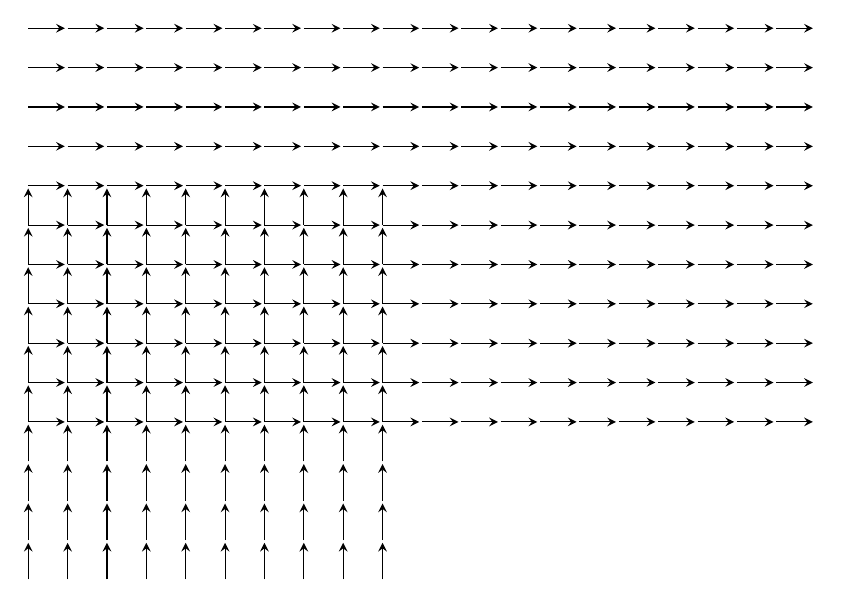
\begin{tikzpicture}[x=0.5cm,y=0.5cm,>=stealth,shorten >=1pt]
\foreach \x in {1,...,10}{
    \foreach \y in {1,...,10}{
	\draw[->] (\x,\y) -- (\x,\y+1);
    }
}
\foreach \x in {1,...,20}{
    \foreach \y in {5,...,15}{
	\draw[->] (\x,\y) -- (\x+1,\y);
    }
}
\end{tikzpicture}
\end{center}
\caption{The relation from \autoref{ex:closure4}}
\label{f:closure4}
\end{figure}
\begin{example}
\label{ex:closure4}
Consider the relation in example {\tt closure4} that comes with
the Omega calculator~\parencite{Omega_calc}, $R = R_1 \cup R_2$,
with
$$
\begin{aligned}
R_1 & = \{\, (x,y) \to (x,y+1) \mid 1 \le x,y \le 10 \,\}
\\
R_2 & = \{\, (x,y) \to (x+1,y) \mid 1 \le x \le 20 \wedge 5 \le y \le 15 \,\}
.
\end{aligned}
$$
This relation is shown graphically in \autoref{f:closure4}.
We have
$$
\begin{aligned}
R_1 \circ R_2 &=
\{\, (x,y) \to (x+1,y+1) \mid 1 \le x \le 9 \wedge 5 \le y \le 10 \,\}
\\
R_2 \circ R_1 &=
\{\, (x,y) \to (x+1,y+1) \mid 1 \le x \le 10 \wedge 4 \le y \le 10 \,\}
.
\end{aligned}
$$
Clearly, $R_1 \circ R_2 \subseteq R_2 \circ R_1$ and so
$$
\left(
R_1 \cup R_2
\right)^+
=
\left(R_2^+ \circ R_1^+\right)
\cup R_1^+
\cup R_2^+
.
$$
\end{example}

\begin{figure}
\newcounter{n}
\newcounter{t1}
\newcounter{t2}
\newcounter{t3}
\newcounter{t4}
\begin{center}
\begin{tikzpicture}[>=stealth,shorten >=1pt]
\setcounter{n}{7}
\foreach \i in {1,...,\value{n}}{
    \foreach \j in {1,...,\value{n}}{
	\setcounter{t1}{2 * \j - 4 - \i + 1}
	\setcounter{t2}{\value{n} - 3 - \i + 1}
	\setcounter{t3}{2 * \i - 1 - \j + 1}
	\setcounter{t4}{\value{n} - \j + 1}
	\ifnum\value{t1}>0\ifnum\value{t2}>0
	\ifnum\value{t3}>0\ifnum\value{t4}>0
	    \draw[thick,->] (\i,\j) to[out=20] (\i+3,\j);
	\fi\fi\fi\fi
	\setcounter{t1}{2 * \j - 1 - \i + 1}
	\setcounter{t2}{\value{n} - \i + 1}
	\setcounter{t3}{2 * \i - 4 - \j + 1}
	\setcounter{t4}{\value{n} - 3 - \j + 1}
	\ifnum\value{t1}>0\ifnum\value{t2}>0
	\ifnum\value{t3}>0\ifnum\value{t4}>0
	    \draw[thick,->] (\i,\j) to[in=-20,out=20] (\i,\j+3);
	\fi\fi\fi\fi
	\setcounter{t1}{2 * \j - 1 - \i + 1}
	\setcounter{t2}{\value{n} - 1 - \i + 1}
	\setcounter{t3}{2 * \i - 1 - \j + 1}
	\setcounter{t4}{\value{n} - 1 - \j + 1}
	\ifnum\value{t1}>0\ifnum\value{t2}>0
	\ifnum\value{t3}>0\ifnum\value{t4}>0
	    \draw[thick,->] (\i,\j) to (\i+1,\j+1);
	\fi\fi\fi\fi
    }
}
\end{tikzpicture}
\end{center}
\caption{The relation from \autoref{ex:decomposition}}
\label{f:decomposition}
\end{figure}
\begin{example}
\label{ex:decomposition}
Consider the relation on the right of \textcite[Figure~2]{Beletska2009},
reproduced in \autoref{f:decomposition}.
The relation can be described as $R = R_1 \cup R_2 \cup R_3$,
with
$$
\begin{aligned}
R_1 &= n \mapsto \{\, (i,j) \to (i+3,j) \mid
i \le 2 j - 4 \wedge
i \le n - 3 \wedge
j \le 2 i - 1 \wedge
j \le n \,\}
\\
R_2 &= n \mapsto \{\, (i,j) \to (i,j+3) \mid
i \le 2 j - 1 \wedge
i \le n \wedge
j \le 2 i - 4 \wedge
j \le n - 3 \,\}
\\
R_3 &= n \mapsto \{\, (i,j) \to (i+1,j+1) \mid
i \le 2 j - 1 \wedge
i \le n - 1 \wedge
j \le 2 i - 1 \wedge
j \le n - 1\,\}
.
\end{aligned}
$$
The figure shows this relation for $n = 7$.
Both
$R_3 \circ R_1 \subseteq R_1 \circ R_3$
and
$R_3 \circ R_2 \subseteq R_2 \circ R_3$,
which the reader can verify using the {\tt iscc} calculator:
\begin{verbatim}
R1 := [n] -> { [i,j] -> [i+3,j] : i <= 2 j - 4 and i <= n - 3 and
                                  j <= 2 i - 1 and j <= n };
R2 := [n] -> { [i,j] -> [i,j+3] : i <= 2 j - 1 and i <= n and
                                  j <= 2 i - 4 and j <= n - 3 };
R3 := [n] -> { [i,j] -> [i+1,j+1] : i <= 2 j - 1 and i <= n - 1 and
                                    j <= 2 i - 1 and j <= n - 1 };
(R1 . R3) - (R3 . R1);
(R2 . R3) - (R3 . R2);
\end{verbatim}
$R_3$ can therefore be moved forward in any path.
For the other two basic relations, we have both
$R_2 \circ R_1 \not\subseteq R_1 \circ R_2$
and
$R_1 \circ R_2 \not\subseteq R_2 \circ R_1$
and so $R_1$ and $R_2$ form a strongly connected component.
By computing the power of $R_3$ and $R_1 \cup R_2$ separately
and composing the results, the power of $R$ can be computed exactly
using \eqref{eq:transitive:singleton}.
As explained by \textcite{Beletska2009}, applying the same formula
to $R$ directly, without a decomposition, would result in
an overapproximation of the power.
\end{example}

\subsection{Partitioning the domains and ranges of $R$}

The algorithm of \autoref{s:power} assumes that the input relation $R$
can be treated as a union of translations.
This is a reasonable assumption if $R$ maps elements of a given
abstract domain to the same domain.
However, if $R$ is a union of relations that map between different
domains, then this assumption no longer holds.
In particular, when an entire dependence graph is encoded
in a single relation, as is done by, e.g.,
\textcite[Section~6.1]{Barthou2000MSE}, then it does not make
sense to look at differences between iterations of different domains.
Now, arguably, a modified Floyd-Warshall algorithm should
be applied to the dependence graph, as advocated by
\textcite{Kelly1996closure}, with the transitive closure operation
only being applied to relations from a given domain to itself.
However, it is also possible to detect disjoint domains and ranges
and to apply Floyd-Warshall internally.

\LinesNumbered
\begin{algorithm}
\caption{The modified Floyd-Warshall algorithm of
\protect\textcite{Kelly1996closure}}
\label{a:Floyd}
\SetKwInput{Input}{Input}
\SetKwInput{Output}{Output}
\Input{Relations $R_{pq}$, $0 \le p, q < n$}
\Output{Updated relations $R_{pq}$ such that each relation
$R_{pq}$ contains all indirect paths from $p$ to $q$ in the input graph}
%
\BlankLine
\SetAlgoVlined
\DontPrintSemicolon
%
\For{$r \in [0, n-1]$}{
    $R_{rr} \coloneqq R_{rr}^+$ \nllabel{l:Floyd:closure}\;
    \For{$p \in [0, n-1]$}{
	\For{$q \in [0, n-1]$}{
	    \If{$p \ne r$ or $q \ne r$}{
		$R_{pq} \coloneqq R_{pq} \cup \left(R_{rq} \circ R_{pr}\right)
			     \cup \left(R_{rq} \circ R_{rr} \circ R_{pr}\right)$
	     \nllabel{l:Floyd:update}
	     }
	}
    }
}
\end{algorithm}

Let the input relation $R$ be a union of $m$ basic relations $R_i$.
Let $D_{2i}$ be the domains of $R_i$ and $D_{2i+1}$ the ranges of $R_i$.
The first step is to group overlapping $D_j$ until a partition is
obtained.  If the resulting partition consists of a single part,
then we continue with the algorithm of \autoref{s:power}.
Otherwise, we apply Floyd-Warshall on the graph with as vertices
the parts of the partition and as edges the $R_i$ attached to
the appropriate pairs of vertices.
In particular, let there be $n$ parts $P_k$ in the partition.
We construct $n^2$ relations
$$
R_{pq} \coloneqq \bigcup_{i \text{ s.t. } \domain R_i \subseteq P_p \wedge
				 \range R_i \subseteq P_q} R_i
,
$$
apply \autoref{a:Floyd} and return the union of all resulting
$R_{pq}$ as the transitive closure of $R$.
Each iteration of the $r$-loop in \autoref{a:Floyd} updates
all relations $R_{pq}$ to include paths that go from $p$ to $r$,
possibly stay there for a while, and then go from $r$ to $q$.
Note that paths that ``stay in $r$'' include all paths that
pass through earlier vertices since $R_{rr}$ itself has been updated
accordingly in previous iterations of the outer loop.
In principle, it would be sufficient to use the $R_{pr}$
and $R_{rq}$ computed in the previous iteration of the
$r$-loop in Line~\ref{l:Floyd:update}.
However, from an implementation perspective, it is easier
to allow either or both of these to have been updated
in the same iteration of the $r$-loop.
This may result in duplicate paths, but these can usually
be removed by coalescing (\autoref{s:coalescing}) the result of the union
in Line~\ref{l:Floyd:update}, which should be done in any case.
The transitive closure in Line~\ref{l:Floyd:closure}
is performed using a recursive call.  This recursive call
includes the partitioning step, but the resulting partition will
usually be a singleton.
The result of the recursive call will either be exact or an
overapproximation.  The final result of Floyd-Warshall is therefore
also exact or an overapproximation.

\begin{figure}
\begin{center}
\begin{tikzpicture}[x=1cm,y=1cm,>=stealth,shorten >=3pt]
\foreach \x/\y in {0/0,1/1,3/2} {
    \fill (\x,\y) circle (2pt);
}
\foreach \x/\y in {0/1,2/2,3/3} {
    \draw (\x,\y) circle (2pt);
}
\draw[->] (0,0) -- (0,1);
\draw[->] (0,1) -- (1,1);
\draw[->] (2,2) -- (3,2);
\draw[->] (3,2) -- (3,3);
\draw[->,dashed] (2,2) -- (3,3);
\draw[->,dotted] (0,0) -- (1,1);
\end{tikzpicture}
\end{center}
\caption{The relation (solid arrows) on the right of Figure~1 of
\protect\textcite{Beletska2009} and its transitive closure}
\label{f:COCOA:1}
\end{figure}
\begin{example}
Consider the relation on the right of Figure~1 of
\textcite{Beletska2009},
reproduced in \autoref{f:COCOA:1}.
This relation can be described as
$$
\begin{aligned}
\{\, (x, y) \to (x_2, y_2) \mid {} & (3y = 2x \wedge x_2 = x \wedge 3y_2 = 3 + 2x \wedge x \ge 0 \wedge x \le 3) \vee {} \\
& (x_2 = 1 + x \wedge y_2 = y \wedge x \ge 0 \wedge 3y \ge 2 + 2x \wedge x \le 2 \wedge 3y \le 3 + 2x) \,\}
.
\end{aligned}
$$
Note that the domain of the upward relation overlaps with the range
of the rightward relation and vice versa, but that the domain
of neither relation overlaps with its own range or the domain of
the other relation.
The domains and ranges can therefore be partitioned into two parts,
$P_0$ and $P_1$, shown as the white and black dots in \autoref{f:COCOA:1},
respectively.
Initially, we have
$$
\begin{aligned}
R_{00} & = \emptyset
\\
R_{01} & = 
\{\, (x, y) \to (x+1, y) \mid 
(x \ge 0 \wedge 3y \ge 2 + 2x \wedge x \le 2 \wedge 3y \le 3 + 2x) \,\}
\\
R_{10} & =
\{\, (x, y) \to (x_2, y_2) \mid (3y = 2x \wedge x_2 = x \wedge 3y_2 = 3 + 2x \wedge x \ge 0 \wedge x \le 3) \,\}
\\
R_{11} & = \emptyset
.
\end{aligned}
$$
In the first iteration, $R_{00}$ remains the same ($\emptyset^+ = \emptyset$).
$R_{01}$ and $R_{10}$ are therefore also unaffected, but
$R_{11}$ is updated to include $R_{01} \circ R_{10}$, i.e.,
the dashed arrow in the figure.
This new $R_{11}$ is obviously transitively closed, so it is not
changed in the second iteration and it does not have an effect
on $R_{01}$ and $R_{10}$.  However, $R_{00}$ is updated to
include $R_{10} \circ R_{01}$, i.e., the dotted arrow in the figure.
The transitive closure of the original relation is then equal to
$R_{00} \cup R_{01} \cup R_{10} \cup R_{11}$.
\end{example}

\subsection{Incremental Computation}
\label{s:incremental}

In some cases it is possible and useful to compute the transitive closure
of union of basic relations incrementally.  In particular,
if $R$ is a union of $m$ basic maps,
$$
R = \bigcup_j R_j
,
$$
then we can pick some $R_i$ and compute the transitive closure of $R$ as
\begin{equation}
\label{eq:transitive:incremental}
R^+ = R_i^+ \cup
\left(
\bigcup_{j \ne i}
R_i^* \circ R_j \circ R_i^*
\right)^+
.
\end{equation}
For this approach to be successful, it is crucial that each
of the disjuncts in the argument of the second transitive
closure in \eqref{eq:transitive:incremental} be representable
as a single basic relation, i.e., without a union.
If this condition holds, then by using \eqref{eq:transitive:incremental},
the number of disjuncts in the argument of the transitive closure
can be reduced by one.
Now, $R_i^* = R_i^+ \cup \identity$, but in some cases it is possible
to relax the constraints of $R_i^+$ to include part of the identity relation,
say on domain $D$.  We will use the notation
${\cal C}(R_i,D) = R_i^+ \cup \identity_D$ to represent
this relaxed version of $R^+$.
\textcite{Kelly1996closure} use the notation $R_i^?$.
${\cal C}(R_i,D)$ can be computed by allowing $k$ to attain
the value $0$ in \eqref{eq:transitive:Q} and by using
$$
P \cap \left(D \to D\right)
$$
instead of \eqref{eq:transitive:approx}.
Typically, $D$ will be a strict superset of both $\domain R_i$
and $\range R_i$.  We therefore need to check that domain
and range of the transitive closure are part of ${\cal C}(R_i,D)$,
i.e., the part that results from the paths of positive length ($k \ge 1$),
are equal to the domain and range of $R_i$.
If not, then the incremental approach cannot be applied for
the given choice of $R_i$ and $D$.

In order to be able to replace $R^*$ by ${\cal C}(R_i,D)$
in \eqref{eq:transitive:incremental}, $D$ should be chosen
to include both $\domain R$ and $\range R$, i.e., such
that $\identity_D \circ R_j \circ \identity_D = R_j$ for all $j\ne i$.
\textcite{Kelly1996closure} say that they use
$D = \domain R_i \cup \range R_i$, but presumably they mean that
they use $D = \domain R \cup \range R$.
Now, this expression of $D$ contains a union, so it not directly usable.
\textcite{Kelly1996closure} do not explain how they avoid this union.
Apparently, in their implementation,
they are using the convex hull of $\domain R \cup \range R$
or at least an approximation of this convex hull.
We use the simple hull (\autoref{s:simple hull}) of $\domain R \cup \range R$.

It is also possible to use a domain $D$ that does {\em not\/}
include $\domain R \cup \range R$, but then we have to
compose with ${\cal C}(R_i,D)$ more selectively.
In particular, if we have
\begin{equation}
\label{eq:transitive:right}
\text{for each $j \ne i$ either }
\domain R_j \subseteq D \text{ or } \domain R_j \cap \range R_i = \emptyset
\end{equation}
and, similarly,
\begin{equation}
\label{eq:transitive:left}
\text{for each $j \ne i$ either }
\range R_j \subseteq D \text{ or } \range R_j \cap \domain R_i = \emptyset
\end{equation}
then we can refine \eqref{eq:transitive:incremental} to
$$
R_i^+ \cup
\left(
\left(
\bigcup_{\shortstack{$\scriptstyle\domain R_j \subseteq D $\\
		     $\scriptstyle\range R_j \subseteq D$}}
{\cal C} \circ R_j \circ {\cal C}
\right)
\cup
\left(
\bigcup_{\shortstack{$\scriptstyle\domain R_j \cap \range R_i = \emptyset$\\
		     $\scriptstyle\range R_j \subseteq D$}}
\!\!\!\!\!
{\cal C} \circ R_j
\right)
\cup
\left(
\bigcup_{\shortstack{$\scriptstyle\domain R_j \subseteq D $\\
		     $\scriptstyle\range R_j \cap \domain R_i = \emptyset$}}
\!\!\!\!\!
R_j \circ {\cal C}
\right)
\cup
\left(
\bigcup_{\shortstack{$\scriptstyle\domain R_j \cap \range R_i = \emptyset$\\
		     $\scriptstyle\range R_j \cap \domain R_i = \emptyset$}}
\!\!\!\!\!
R_j
\right)
\right)^+
.
$$
If only property~\eqref{eq:transitive:right} holds,
we can use
$$
R_i^+ \cup
\left(
\left(
R_i^+ \cup \identity
\right)
\circ
\left(
\left(
\bigcup_{\shortstack{$\scriptstyle\domain R_j \subseteq D $}}
R_j \circ {\cal C}
\right)
\cup
\left(
\bigcup_{\shortstack{$\scriptstyle\domain R_j \cap \range R_i = \emptyset$}}
\!\!\!\!\!
R_j
\right)
\right)^+
\right)
,
$$
while if only property~\eqref{eq:transitive:left} holds,
we can use
$$
R_i^+ \cup
\left(
\left(
\left(
\bigcup_{\shortstack{$\scriptstyle\range R_j \subseteq D $}}
{\cal C} \circ R_j
\right)
\cup
\left(
\bigcup_{\shortstack{$\scriptstyle\range R_j \cap \domain R_i = \emptyset$}}
\!\!\!\!\!
R_j
\right)
\right)^+
\circ
\left(
R_i^+ \cup \identity
\right)
\right)
.
$$

It should be noted that if we want the result of the incremental
approach to be transitively closed, then we can only apply it
if all of the transitive closure operations involved are exact.
If, say, the second transitive closure in \eqref{eq:transitive:incremental}
contains extra elements, then the result does not necessarily contain
the composition of these extra elements with powers of $R_i$.

\subsection{An {\tt Omega}-like implementation}

While the main algorithm of \textcite{Kelly1996closure} is
designed to compute and underapproximation of the transitive closure,
the authors mention that they could also compute overapproximations.
In this section, we describe our implementation of an algorithm
that is based on their ideas.
Note that the {\tt Omega} library computes underapproximations
\parencite[Section 6.4]{Omega_lib}.

The main tool is Equation~(2) of \textcite{Kelly1996closure}.
The input relation $R$ is first overapproximated by a ``d-form'' relation
$$
\{\, \vec i \to \vec j \mid \exists \vec \alpha :
\vec L \le \vec j - \vec i \le \vec U
\wedge
(\forall p : j_p - i_p = M_p \alpha_p)
\,\}
,
$$
where $p$ ranges over the dimensions and $\vec L$, $\vec U$ and
$\vec M$ are constant integer vectors.  The elements of $\vec U$
may be $\infty$, meaning that there is no upper bound corresponding
to that element, and similarly for $\vec L$.
Such an overapproximation can be obtained by computing strides,
lower and upper bounds on the difference set $\Delta \, R$.
The transitive closure of such a ``d-form'' relation is
\begin{equation}
\label{eq:omega}
\{\, \vec i \to \vec j \mid \exists \vec \alpha, k :
k \ge 1 \wedge
k \, \vec L \le \vec j - \vec i \le k \, \vec U
\wedge
(\forall p : j_p - i_p = M_p \alpha_p)
\,\}
.
\end{equation}
The domain and range of this transitive closure are then
intersected with those of the input relation.
This is a special case of the algorithm in \autoref{s:power}.

In their algorithm for computing lower bounds, the authors
use the above algorithm as a substep on the disjuncts in the relation.
At the end, they say
\begin{quote}
If an upper bound is required, it can be calculated in a manner
similar to that of a single conjunct [sic] relation.
\end{quote}
Presumably, the authors mean that a ``d-form'' approximation
of the whole input relation should be used.
However, the accuracy can be improved by also trying to
apply the incremental technique from the same paper,
which is explained in more detail in \autoref{s:incremental}.
In this case, ${\cal C}(R_i,D)$ can be obtained by
allowing the value zero for $k$ in \eqref{eq:omega},
i.e., by computing
$$
\{\, \vec i \to \vec j \mid \exists \vec \alpha, k :
k \ge 0 \wedge
k \, \vec L \le \vec j - \vec i \le k \, \vec U
\wedge
(\forall p : j_p - i_p = M_p \alpha_p)
\,\}
.
$$
In our implementation we take as $D$ the simple hull
(\autoref{s:simple hull}) of $\domain R \cup \range R$.
To determine whether it is safe to use ${\cal C}(R_i,D)$,
we check the following conditions, as proposed by
\textcite{Kelly1996closure}:
${\cal C}(R_i,D) - R_i^+$ is not a union and for each $j \ne i$
the condition
$$
\left({\cal C}(R_i,D) - R_i^+\right)
\circ
R_j
\circ
\left({\cal C}(R_i,D) - R_i^+\right)
=
R_j
$$
holds.


\section{Publications}

\subsection{Publications about the Library}

This is a list of some reports and publications explaining
details of parts of the \ai[\tt]{barvinok} library.

\begin{itemize}
\item \citetitleN{Verdoolaege2004embedded}
\item \citetitleN{Verdoolaege2004TR}
\item \citetitleN{Seghir2004analytical}
\item \citetitleN{Verdoolaege2004analytical}
\item \citetitleN{Verdoolaege2004experiences}
\item \citetitleN{Verdoolaege2005experiences}
\item \citetitleN{Verdoolaege2005barvinok}
\item \citetitleN{Verdoolaege2005PhD}
\item \citetitleN{CFGV06}
\item \citetitleN{Verdoolaege2008counting}
\item \citetitleN{Verdoolaege2007parametric}
\item \citetitleN{Meister2008}
\item \citetitleN{Devos2007}
\item \citetitleN{Koeppe2008parametric}
\item \citetitleN{Koeppe2008implementation}
\item \citetitleN{Verdoolaege2008weighted}
\end{itemize}

\subsection{Publications Refering to the Library}

This is a list of some reports and publications refering to
the \ai[\tt]{barvinok} library.

\begin{itemize}
\item \citetitleN{Beck2009Brion}
\item \citetitleN{Beyls2005hints}
\item \citetitleN{Lasserre2005alternative}
\item \citetitleN{Rabl2006}
\item \citetitleN{Verdoolaege2006odes}
\item \citetitleN{Barvinok2006simplex}
\item \citetitleN{Seghir2006memory}
\item \citetitleN{Pop06}
\item \citetitleN{Baldoni2006}
\item \citetitleN{Koeppe2006primal}
\item \citetitleN{Verdoolaege2007pn}
\item \citetitleN{vanHerick2007}
\item \citetitleN{Lepelley2008}
\item \citetitleN{Berline2006local}
\item \citetitleN{Fukuda2008}
\item \citetitleN{Beck2010}
\item \citetitleN{Aspinall2010}
\item \citetitleN{Koeppe2010}
\item \citetitleN{Ryan2010}
\item \citetitleN{Hubler2012}
\item \citetitleN{Klebanov2014}
\end{itemize}


\bibliography{barvinok}
\bibliographystyle{chicago}

\printglosstex(acr)

\index{index|(}

\let\savesection\section
\def\section#1#2{\savesection#1#2\addcontentsline{toc}{section}{\indexname}}
\printindex
\let\section\savesection

\index{index|)}

\end{document}
